% -*- root: ../Presentation.tex -*-
\section{Analyse af steganografi}
\begin{frame}{Analyse af steganografi}{}
	Metoder brugt til analyse af steganografi:
	\begin{itemize}
		\item Farvehistogram
		\item Sammenligning med original billede
		\item LSB forstærkning
		\item Steganografisk signatur
		\item Brute-decoding
	\end{itemize}
\end{frame}

\begin{frame}{Farvehistogram}{}
\begin{figure}
\centering     %%% not \center
\subfigure[Original]{\label{fig:Room}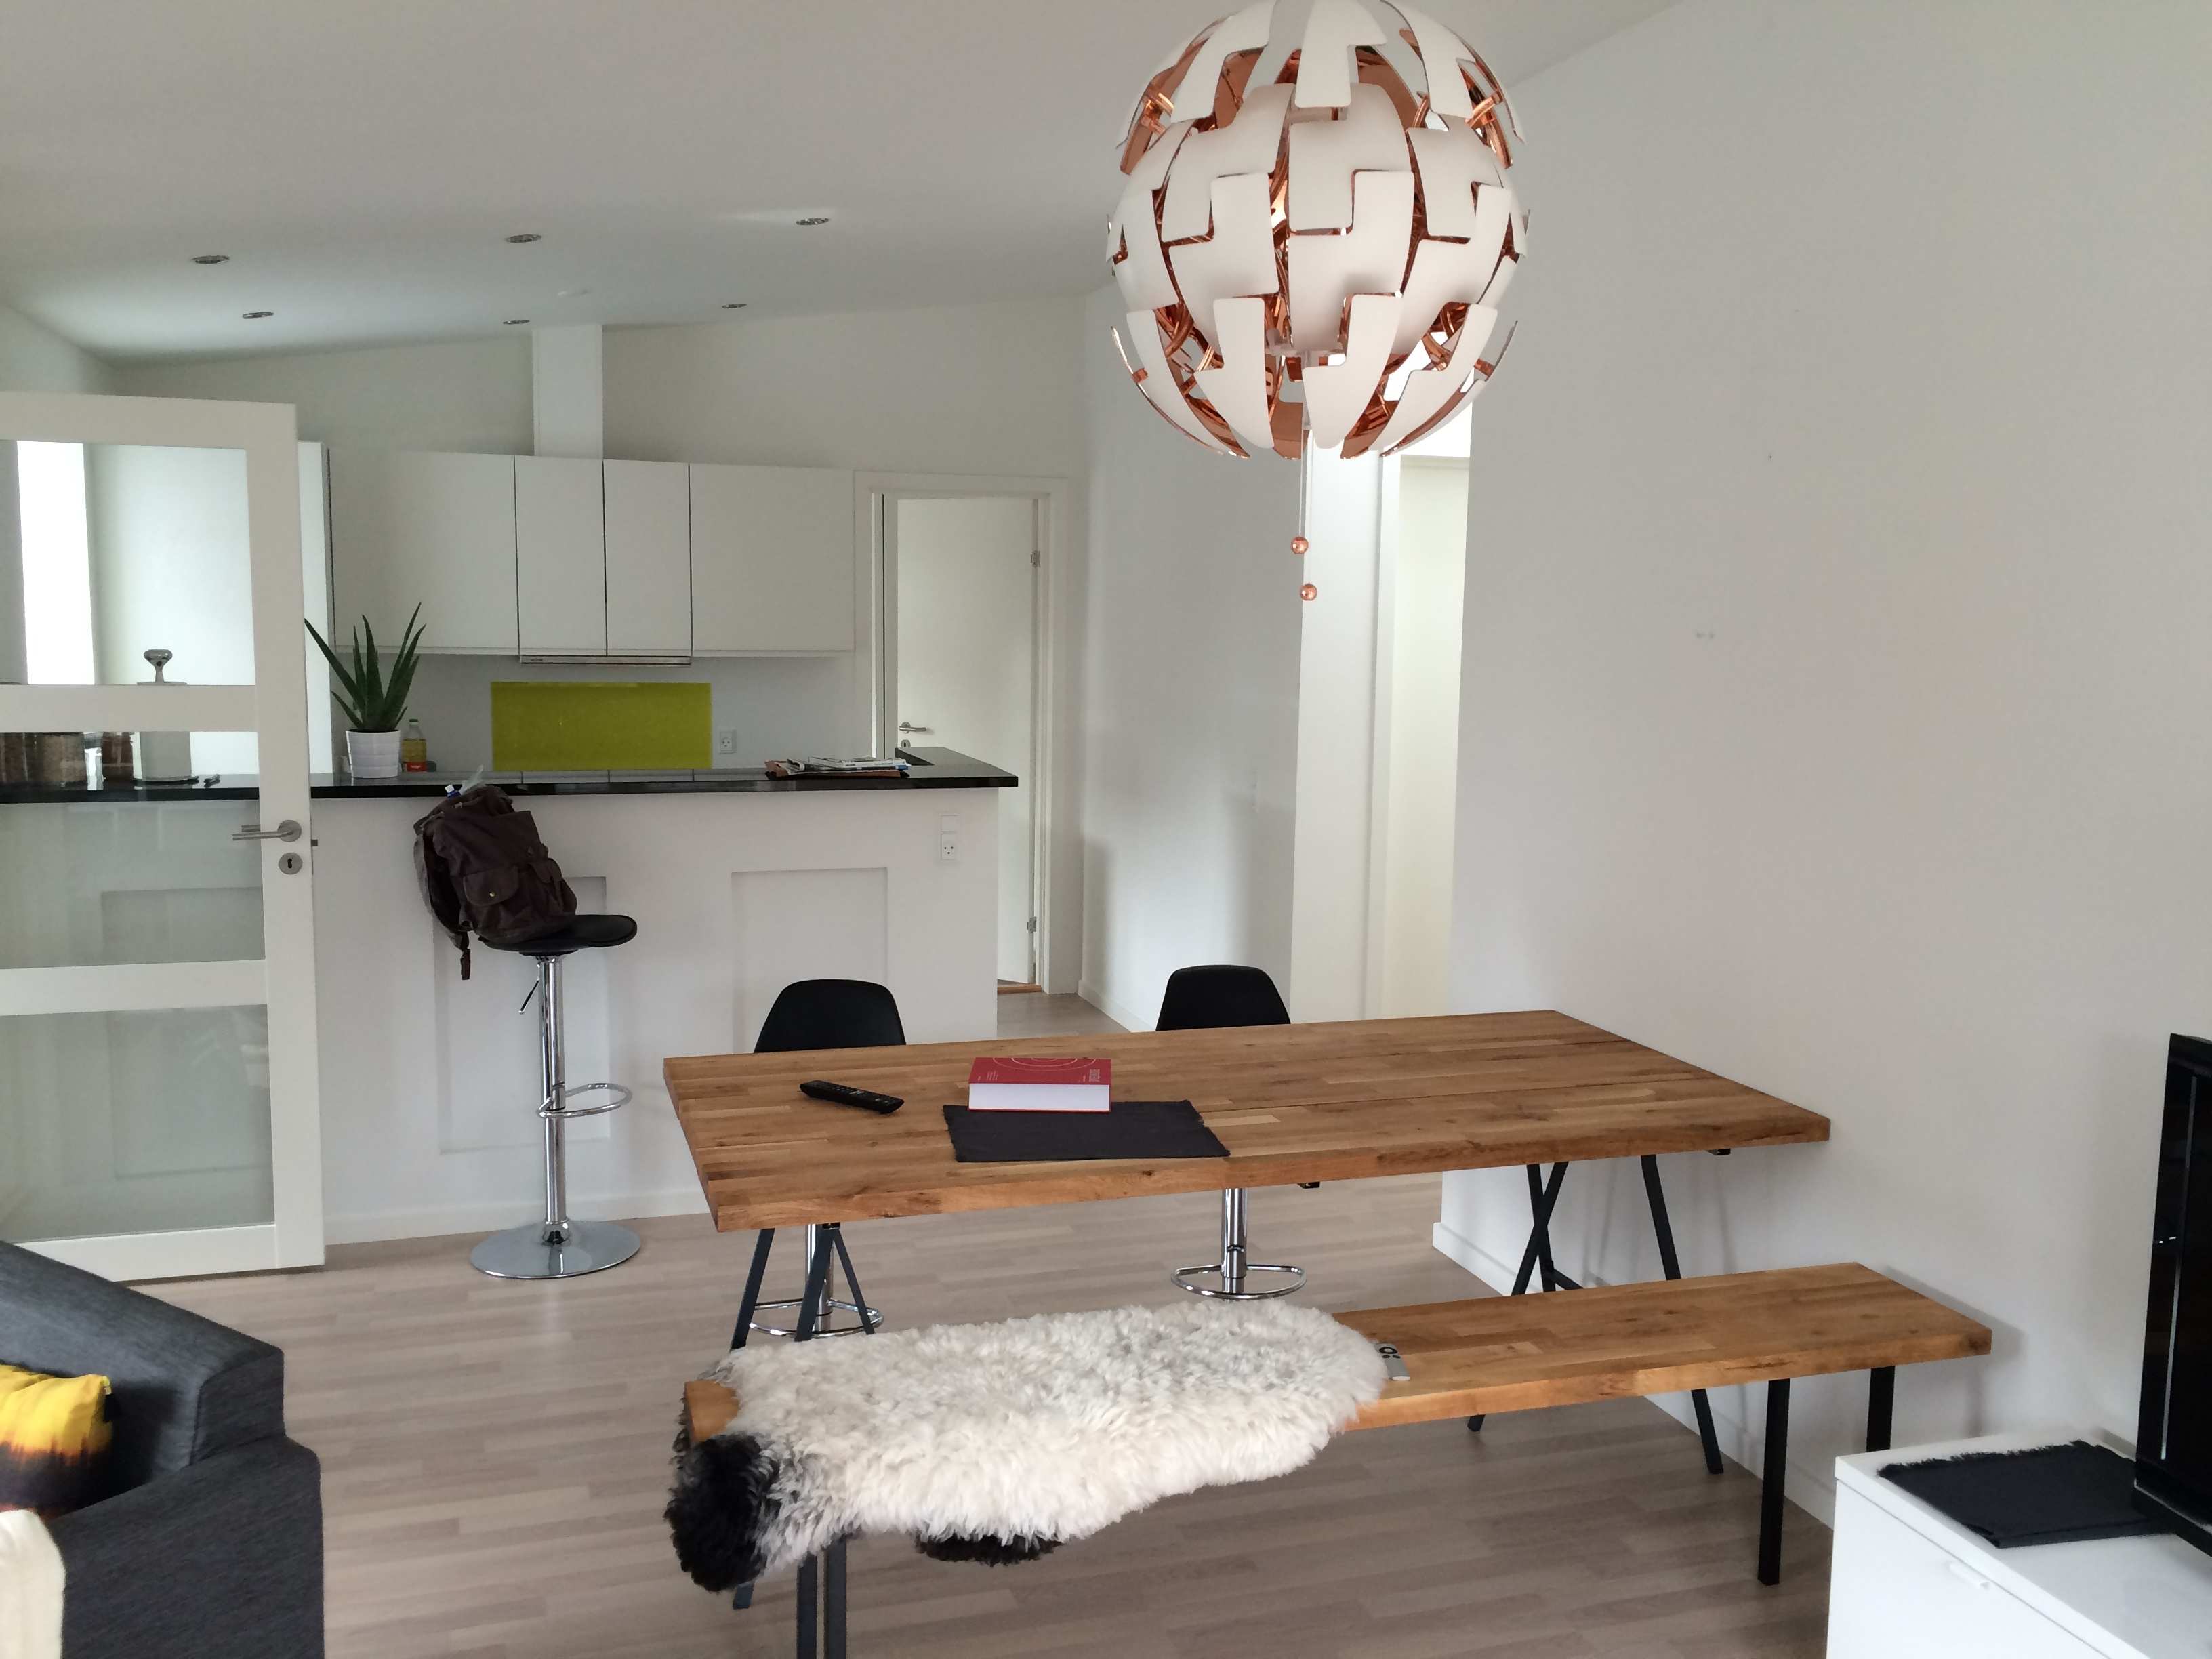
\includegraphics[width=.4\textwidth]{figures/roomOriginal.jpg}}
\end{figure}
\begin{figure}
\centering
\subfigure[0 bytes data gemt]{\label{fig:Room1char}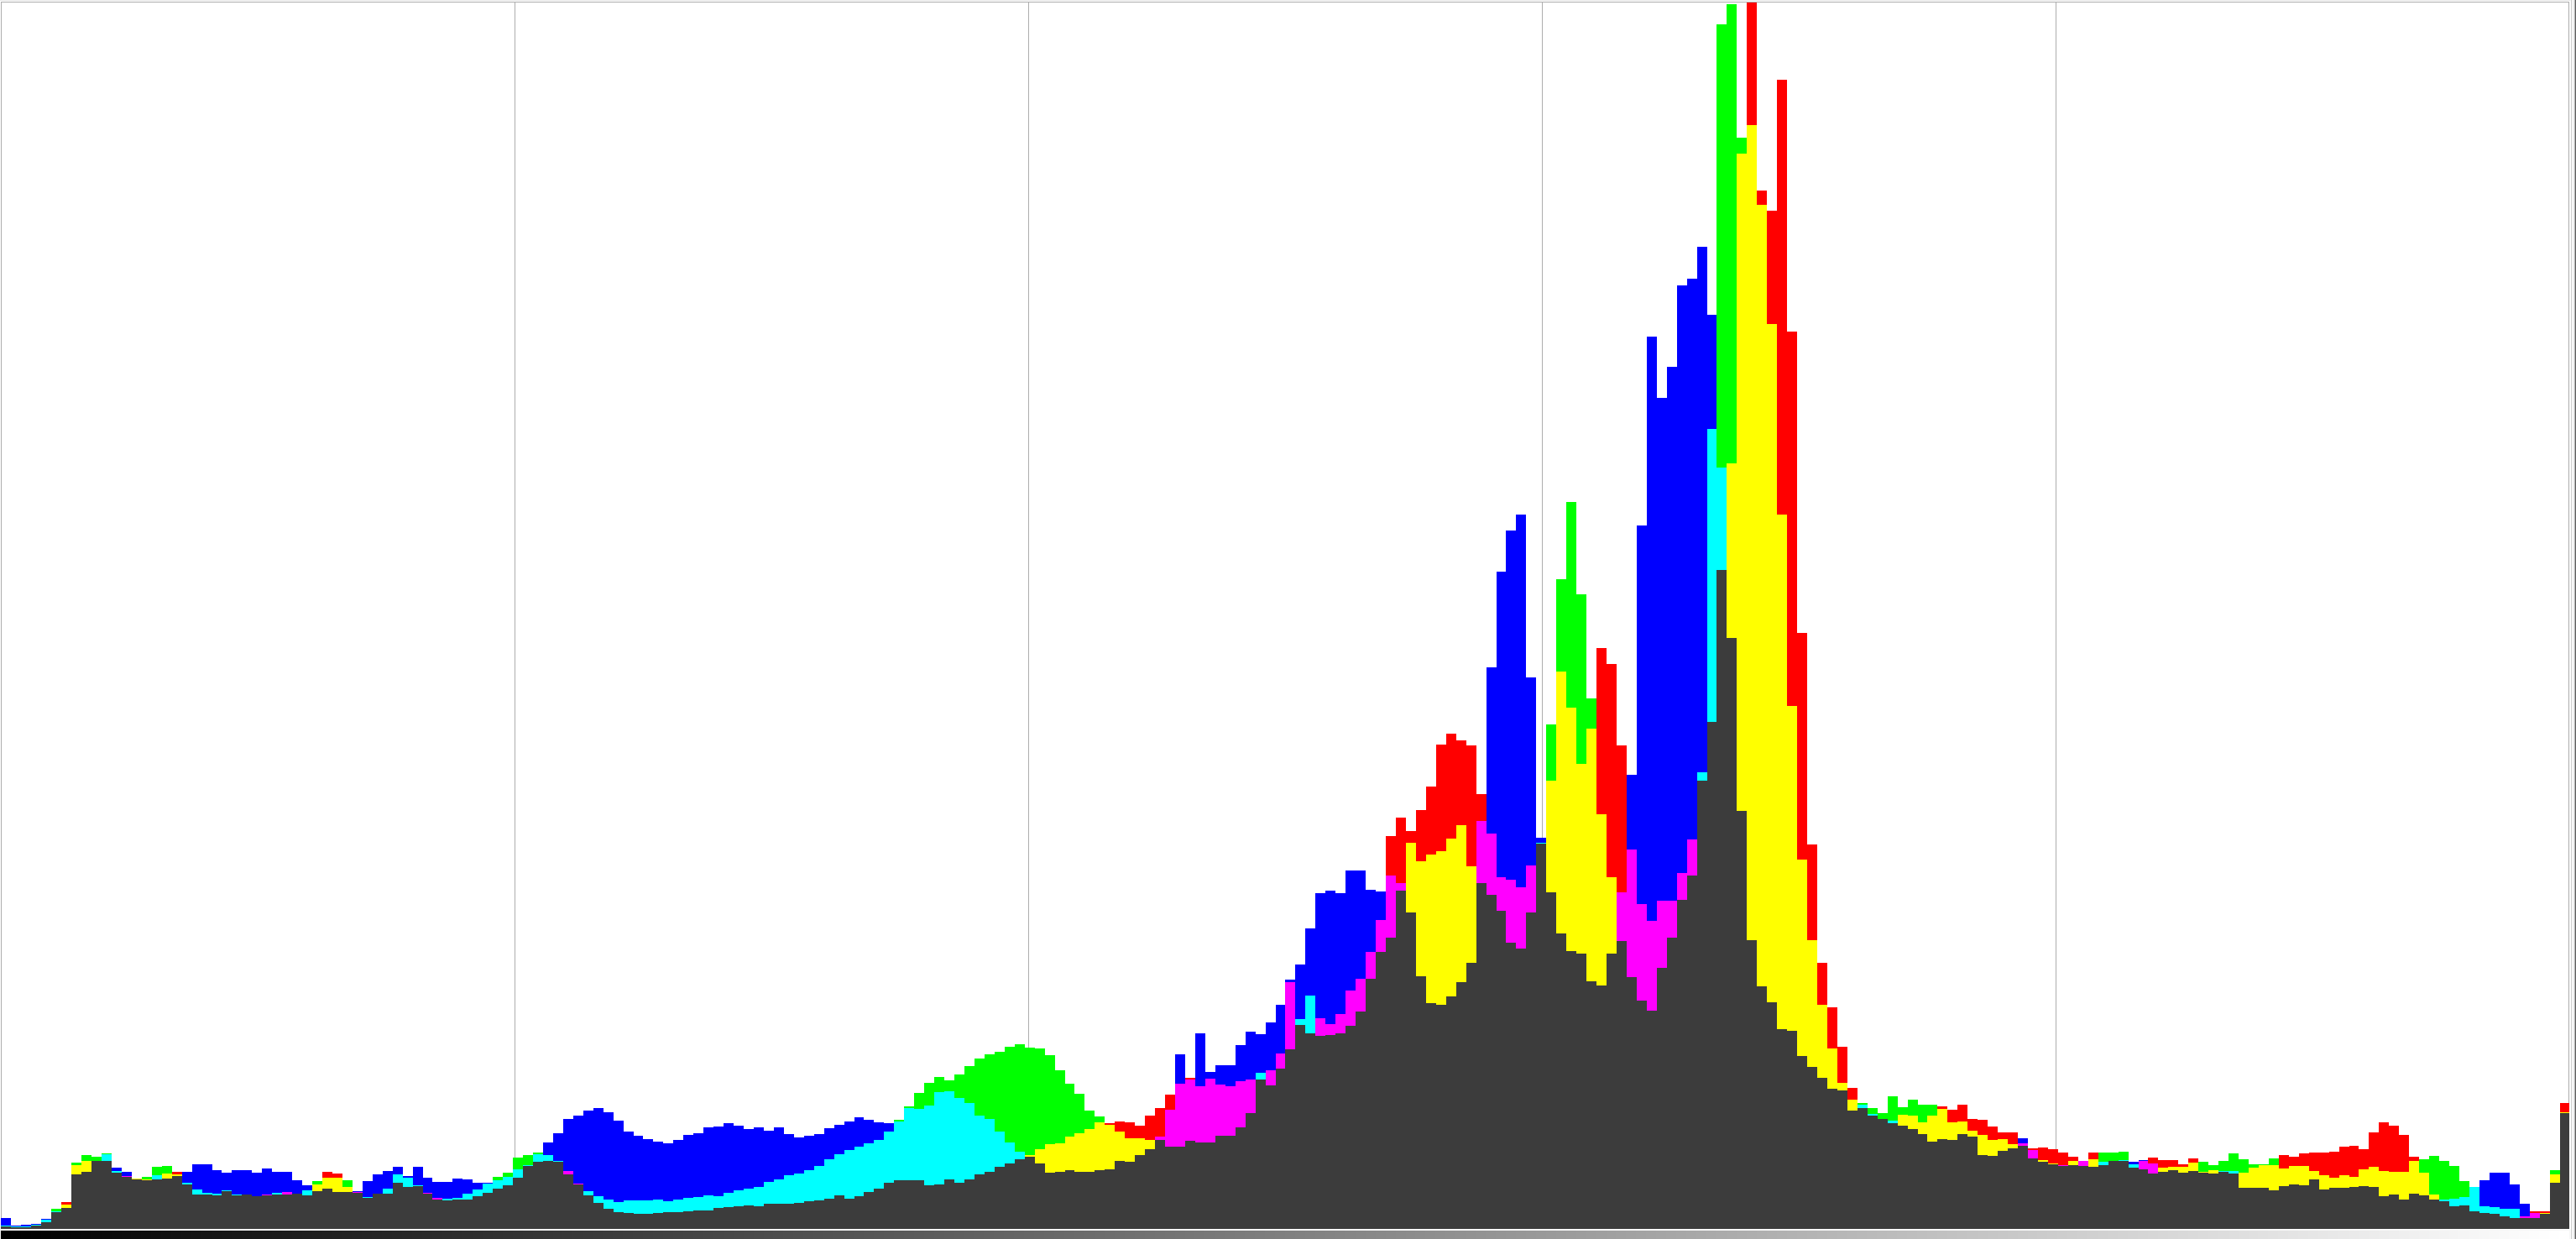
\includegraphics[width=.4\textwidth]{figures/room1char.png}}
\subfigure[2896 bytes data gemt]{\label{fig:RoomIntro}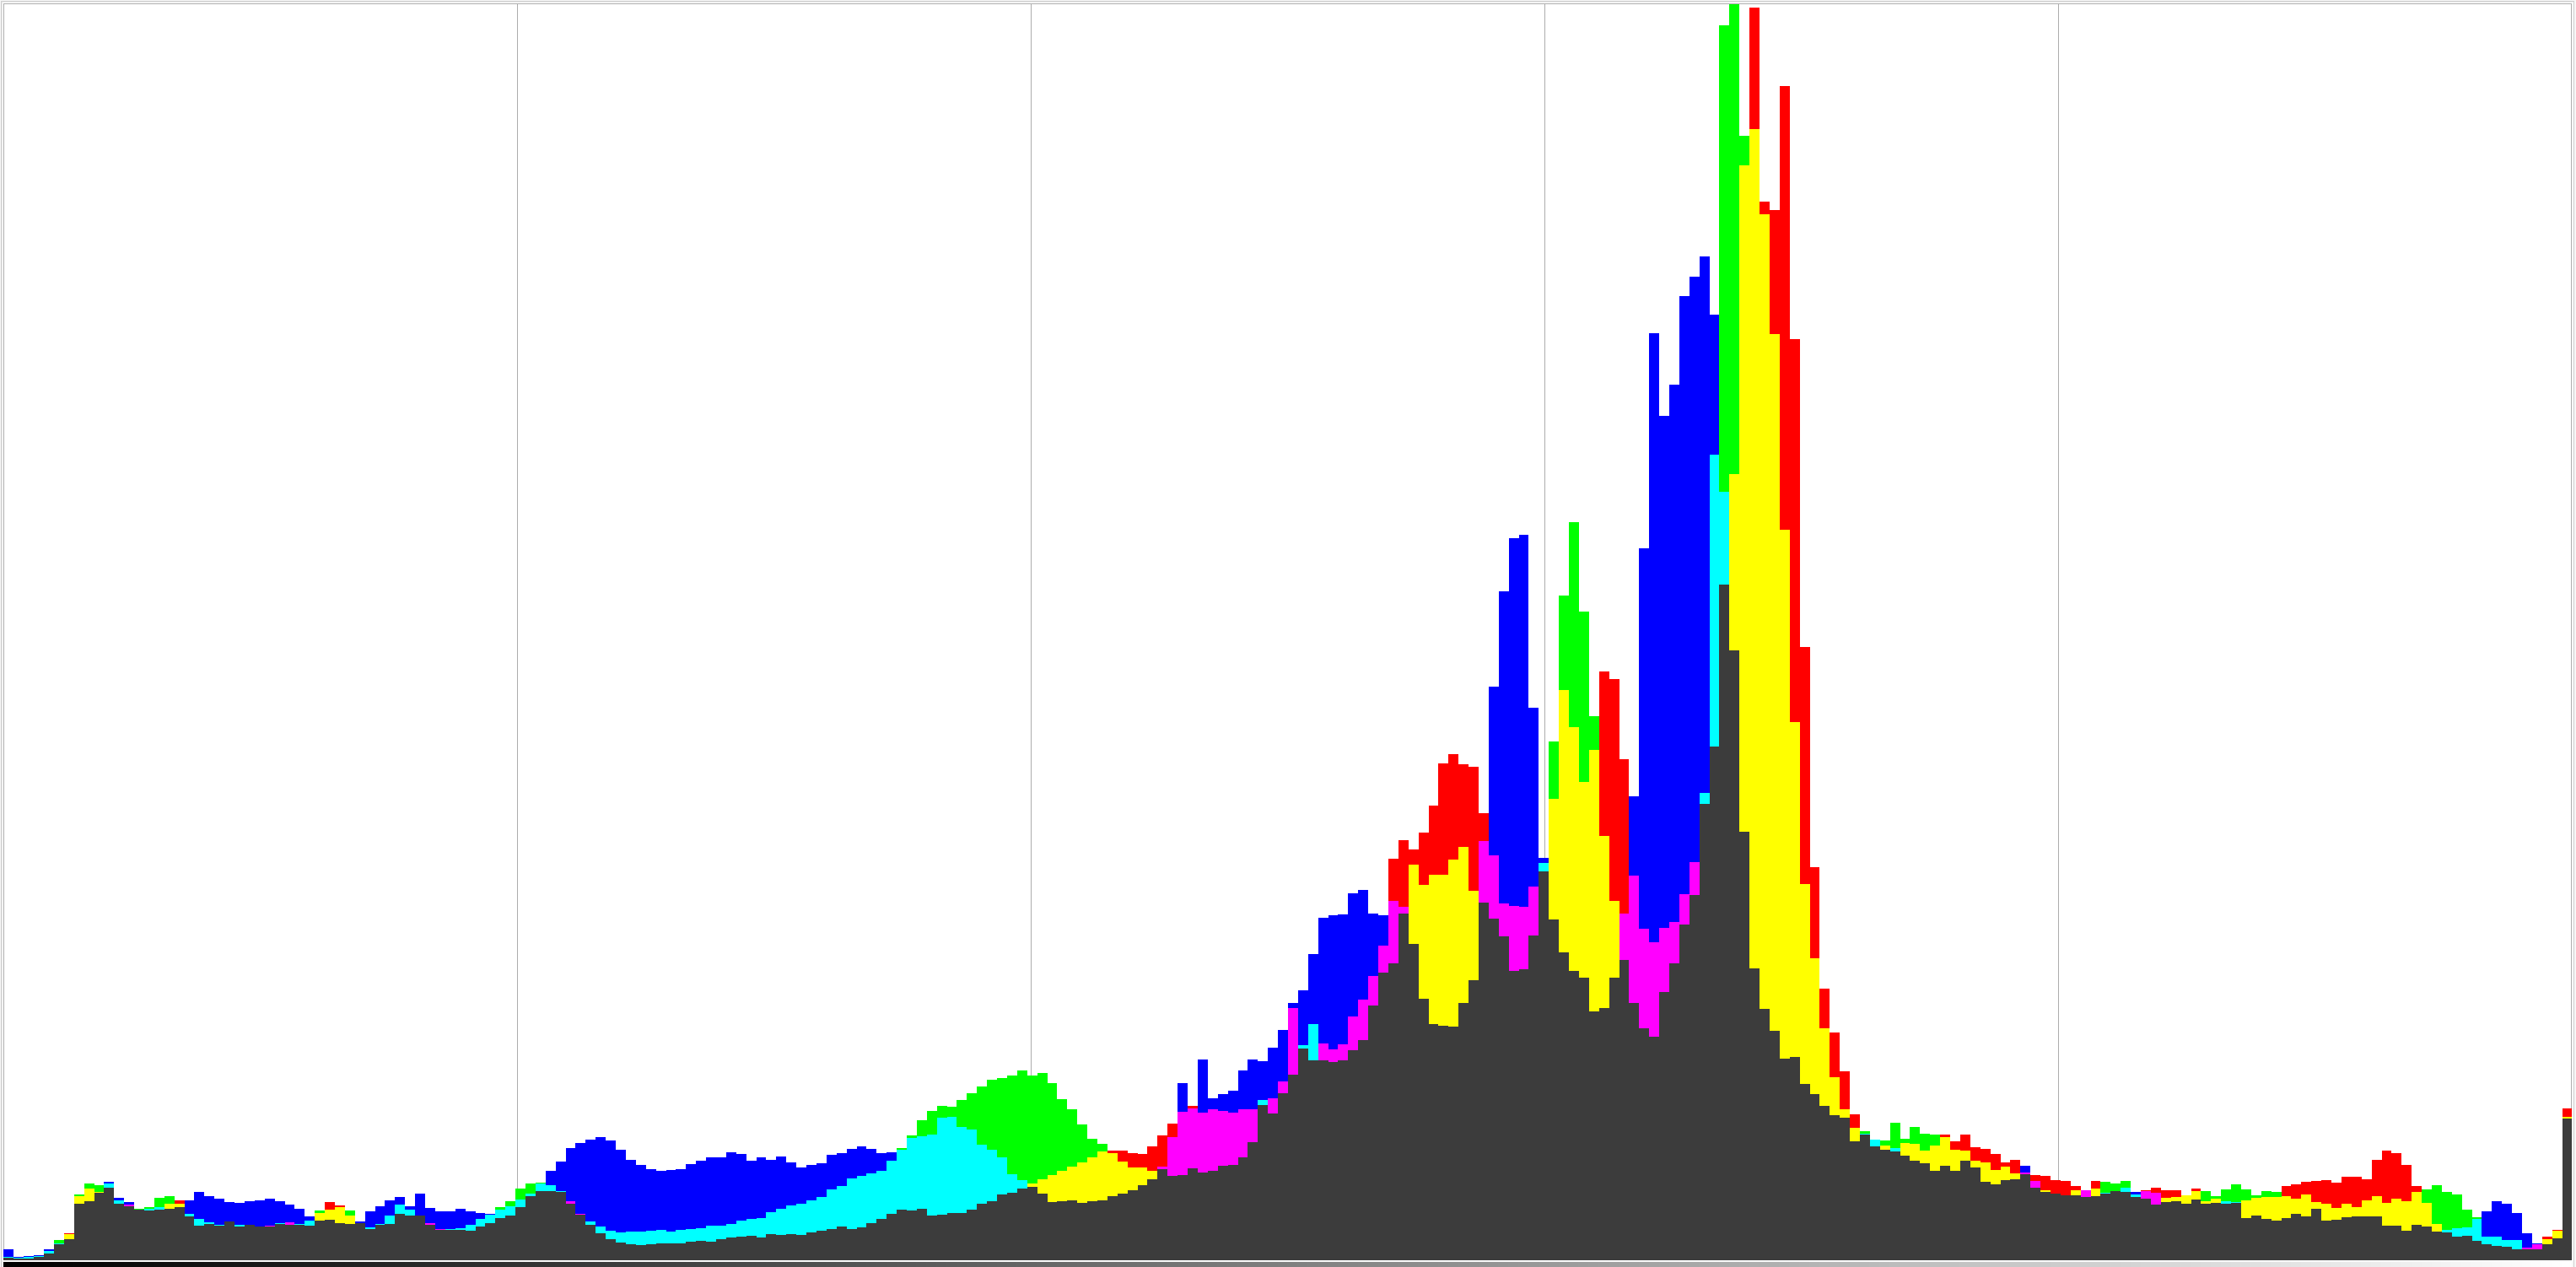
\includegraphics[width=.4\textwidth]{figures/roomEncodedIntroToSteg.png}}
\caption{Sammenligning af farvehistogram}
\end{figure}
\note{Small or no changes to histogram
Not able to detect our program}
\end{frame}

\begin{frame}{Sammenligning med original billede}
\begin{figure}
\centering
\subfigure[Original]{\label{fig:a}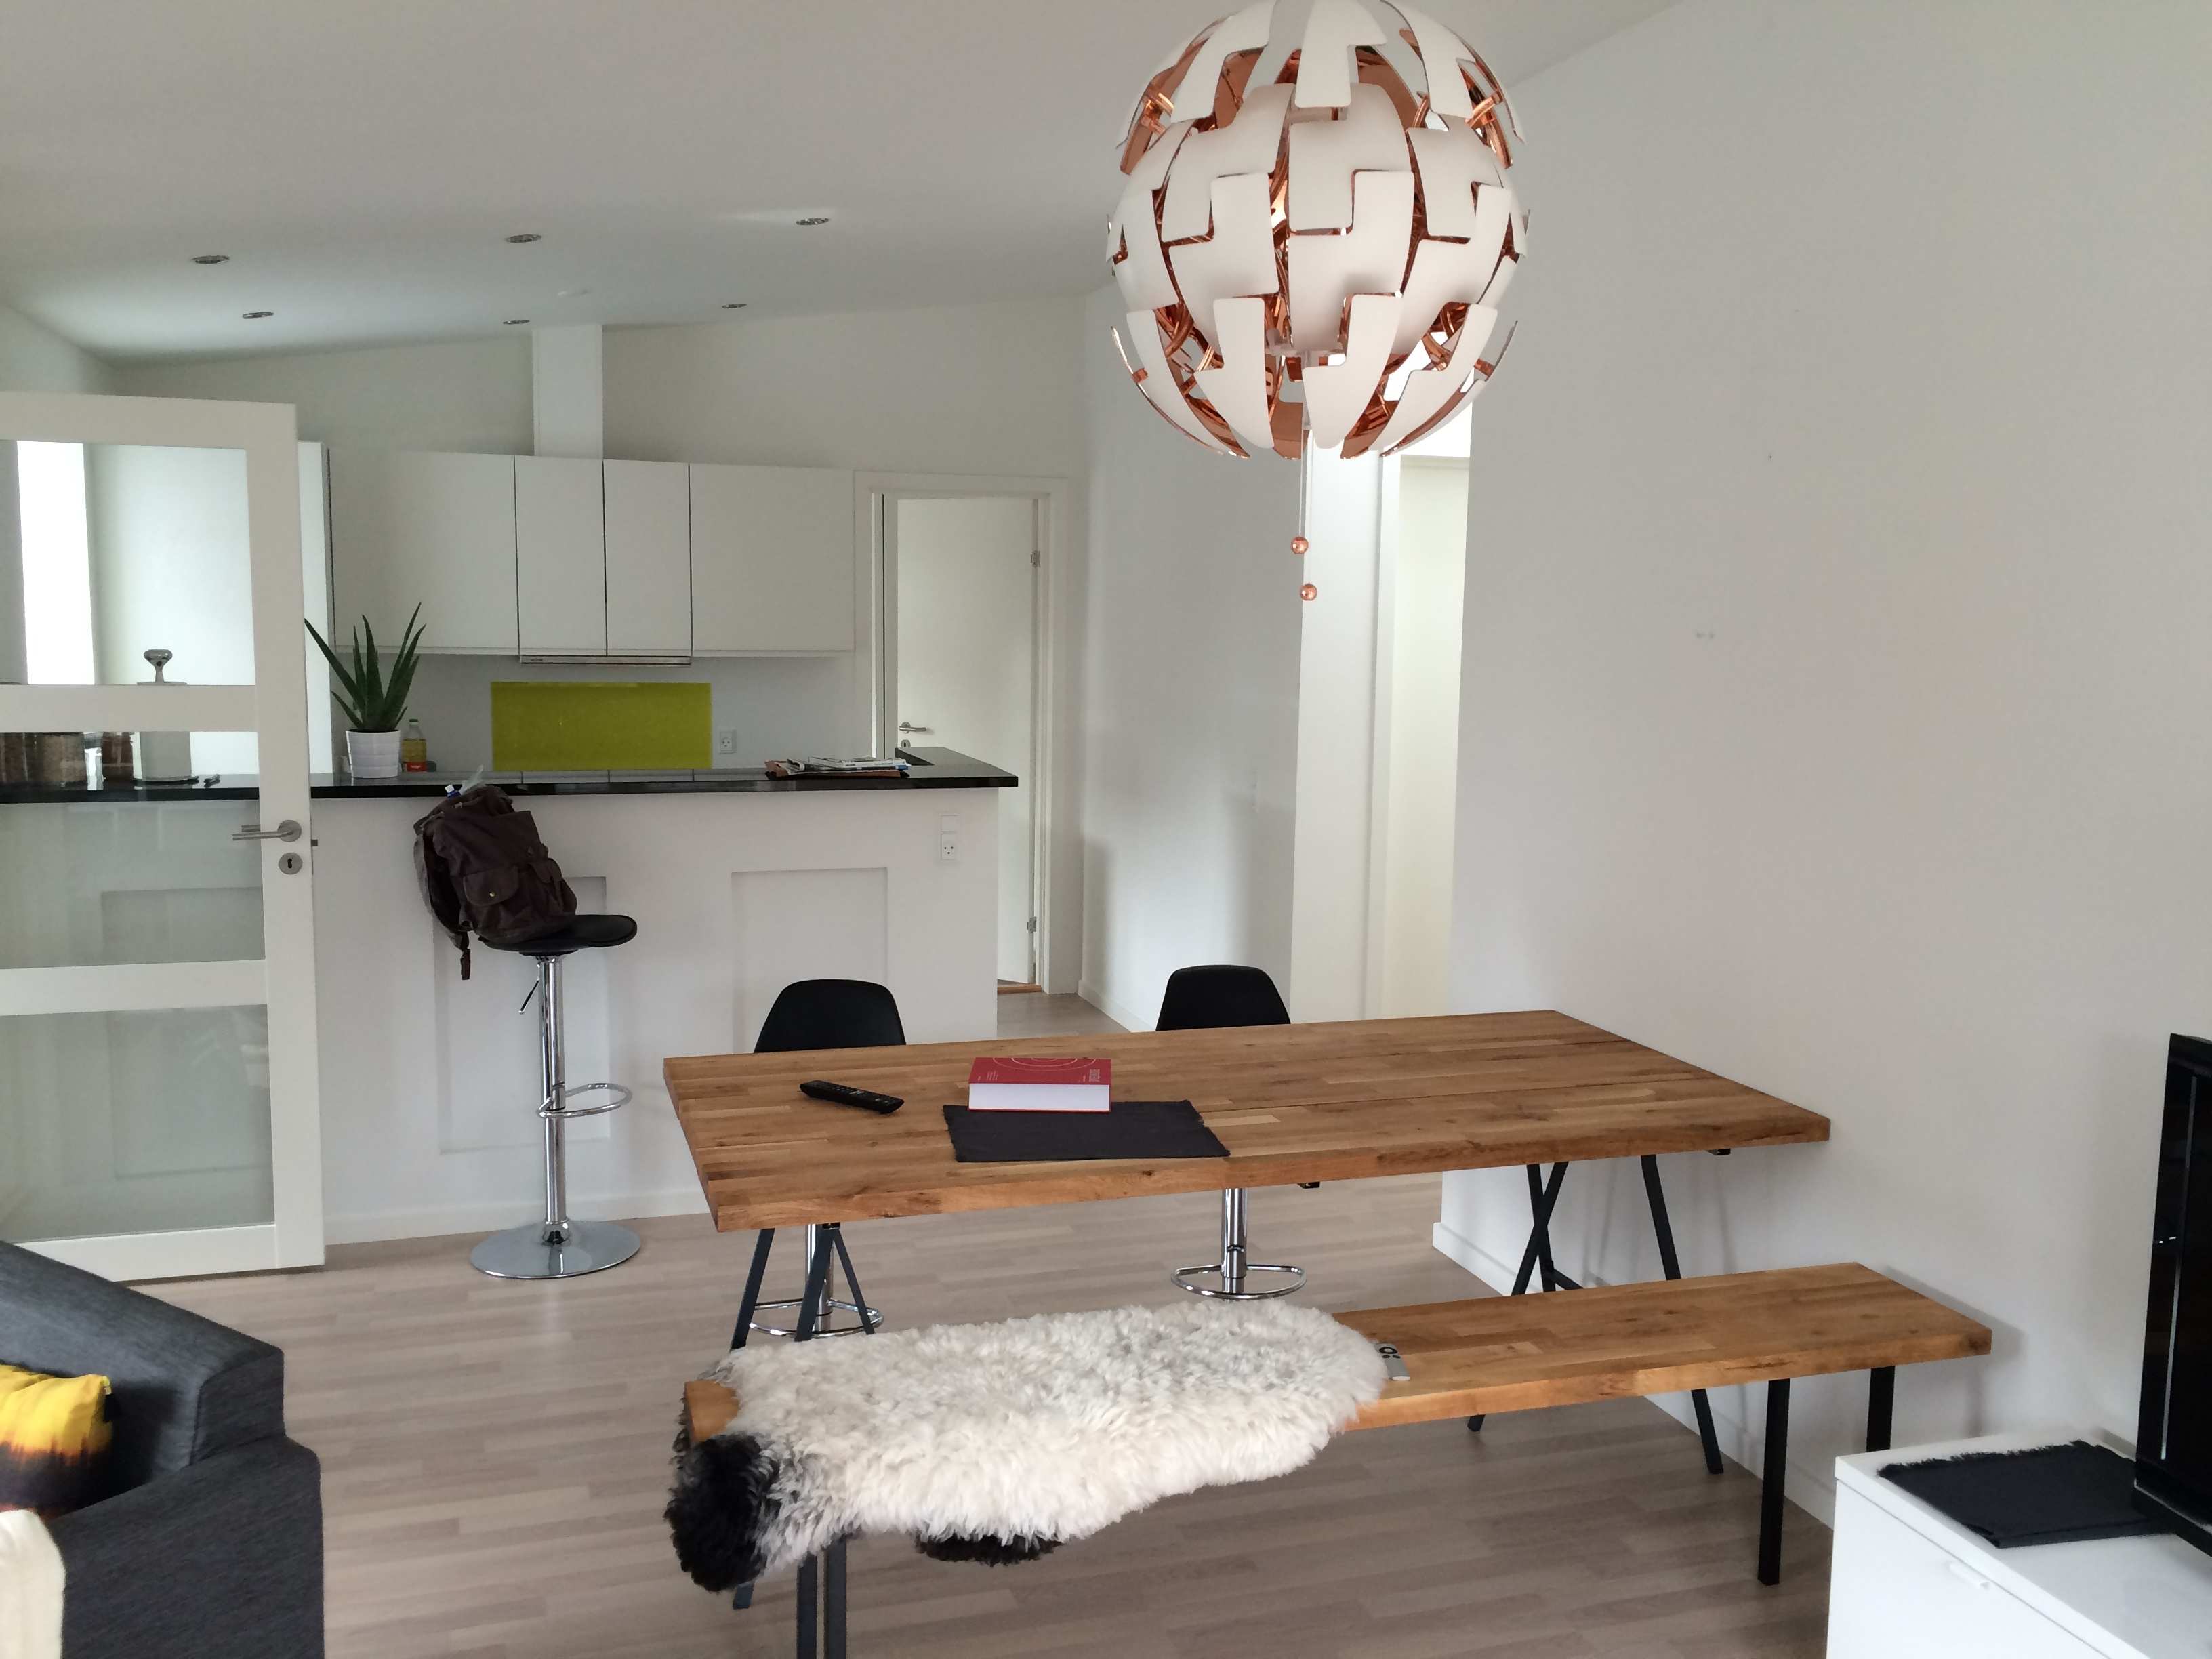
\includegraphics[width=.3\textwidth]{figures/roomOriginal.jpg}}
\end{figure}
\begin{figure}
\centering
\subfigure[2896 bytes vs. original]{\label{fig:b}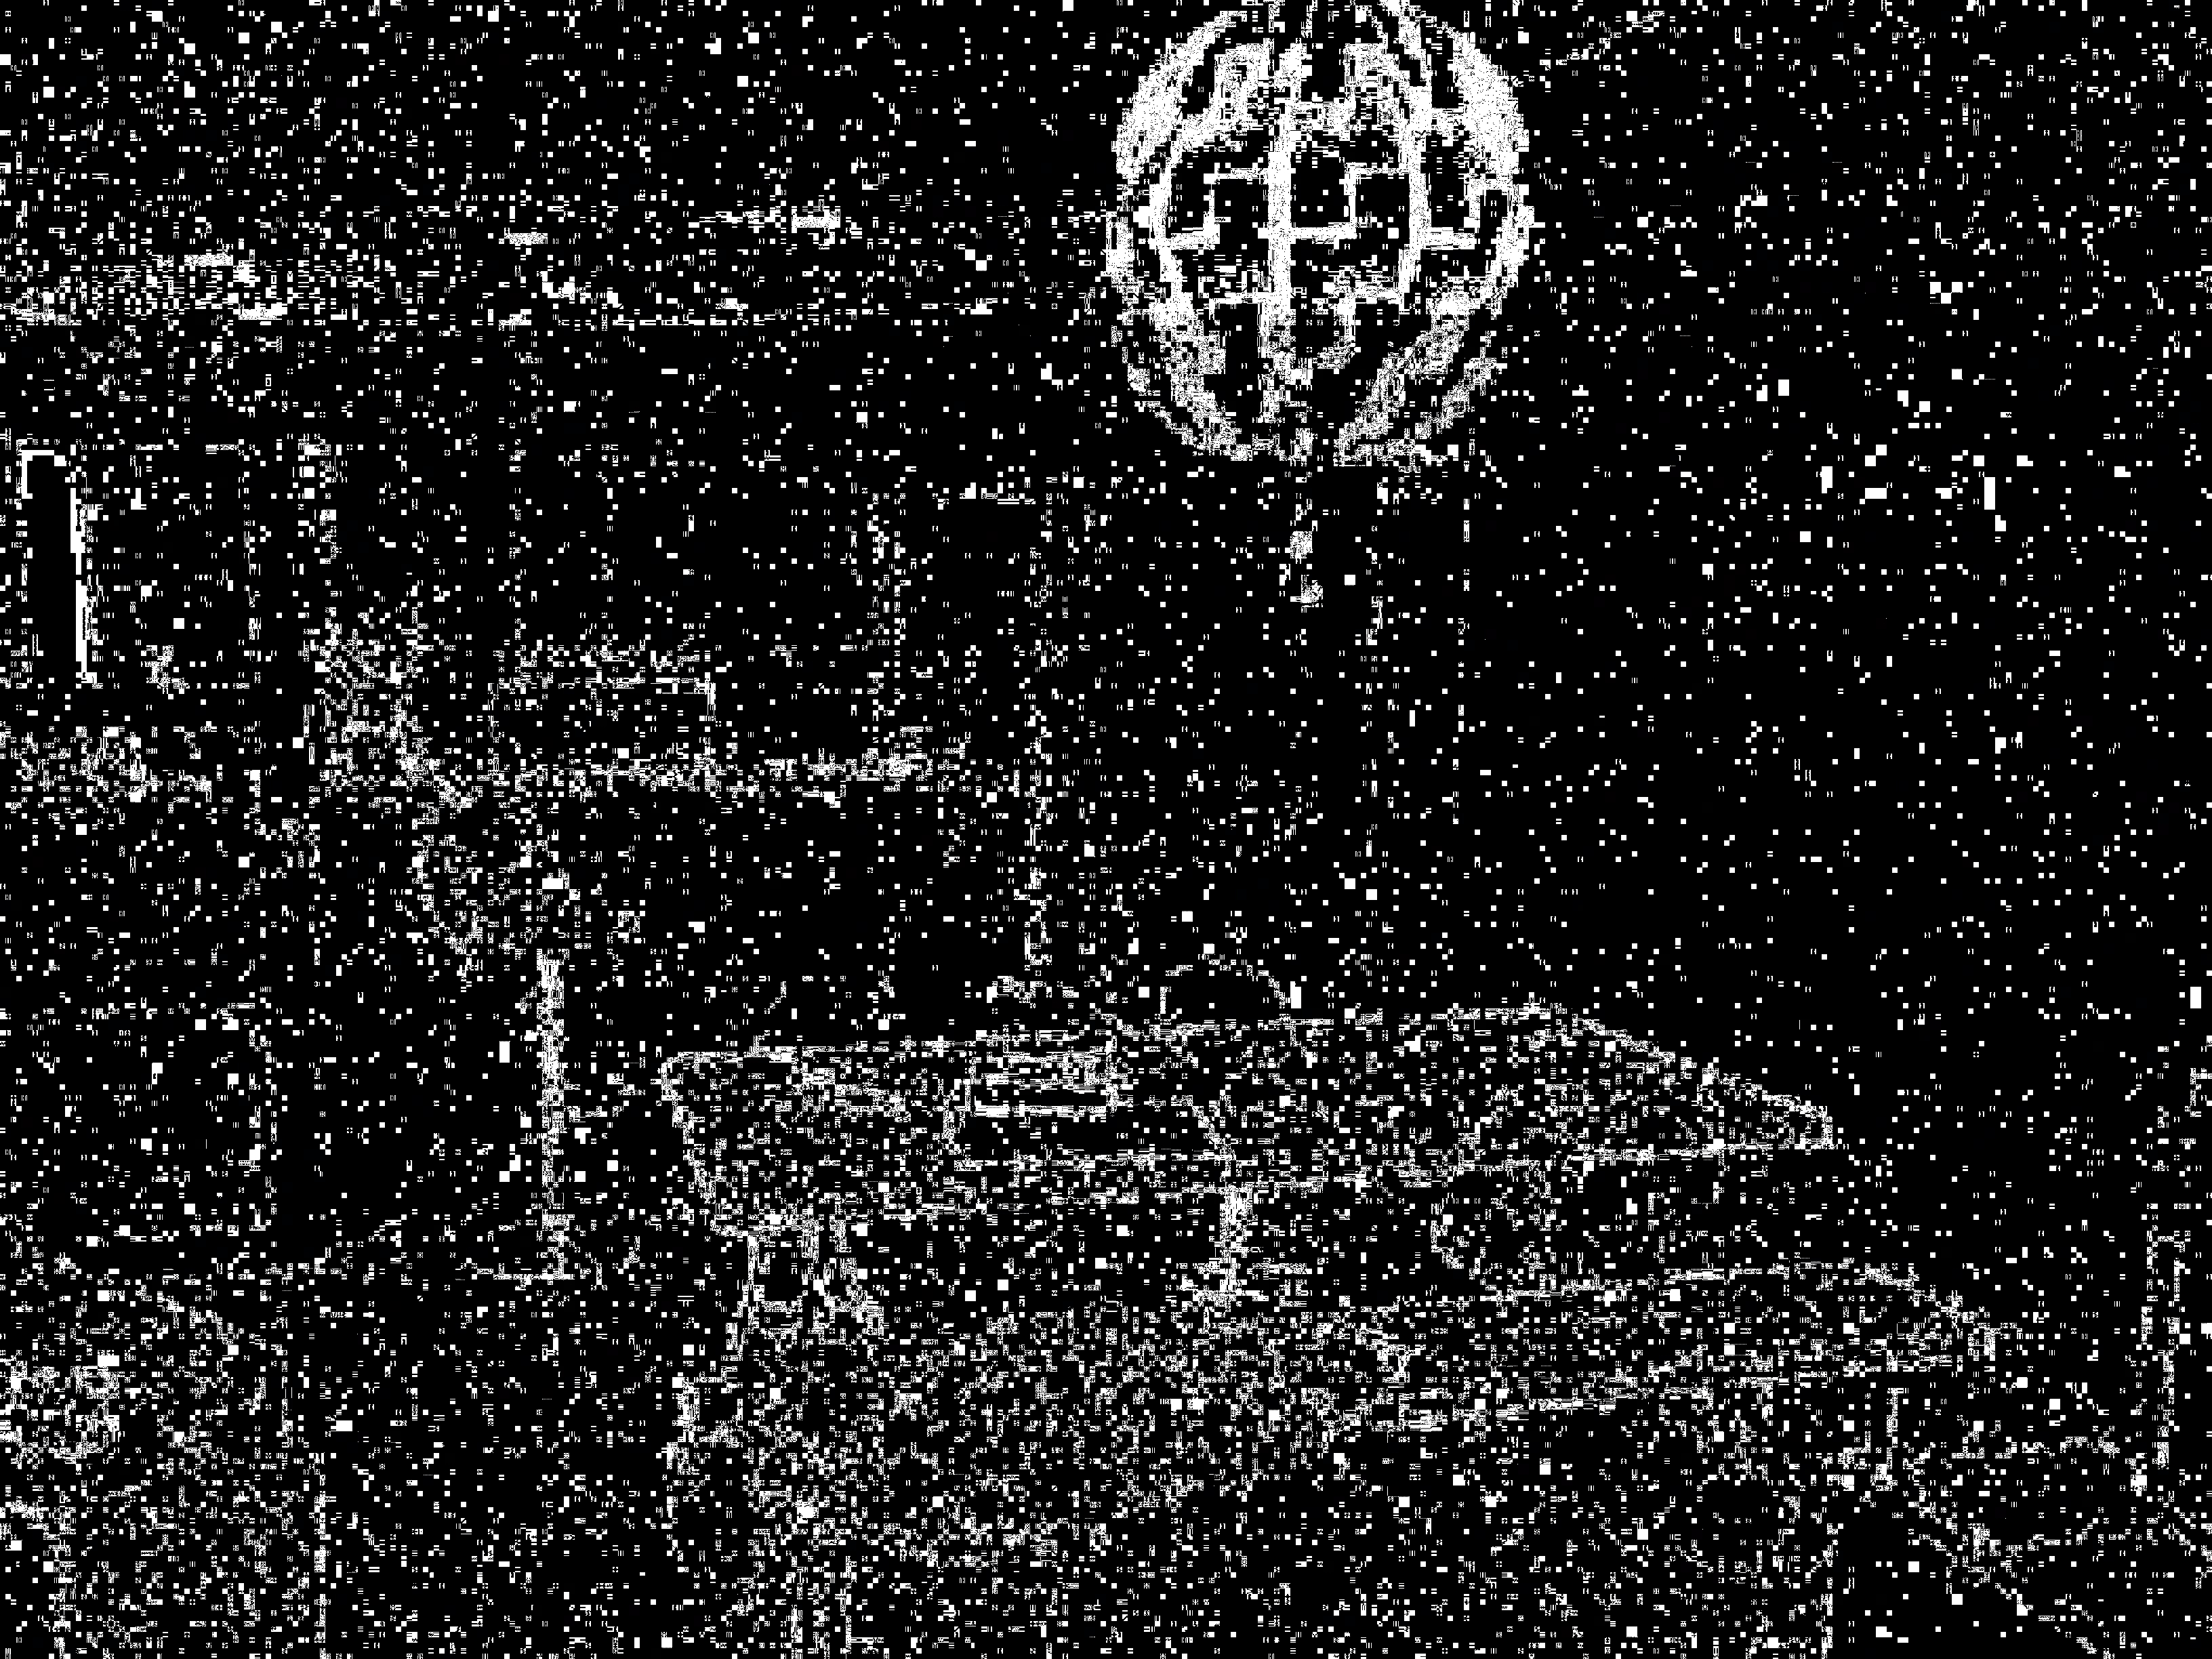
\includegraphics[width=.35\textwidth]{figures/introToStegovs1chardiff.jpg}}
\subfigure[500 bytes vs. original]{\label{fig:a}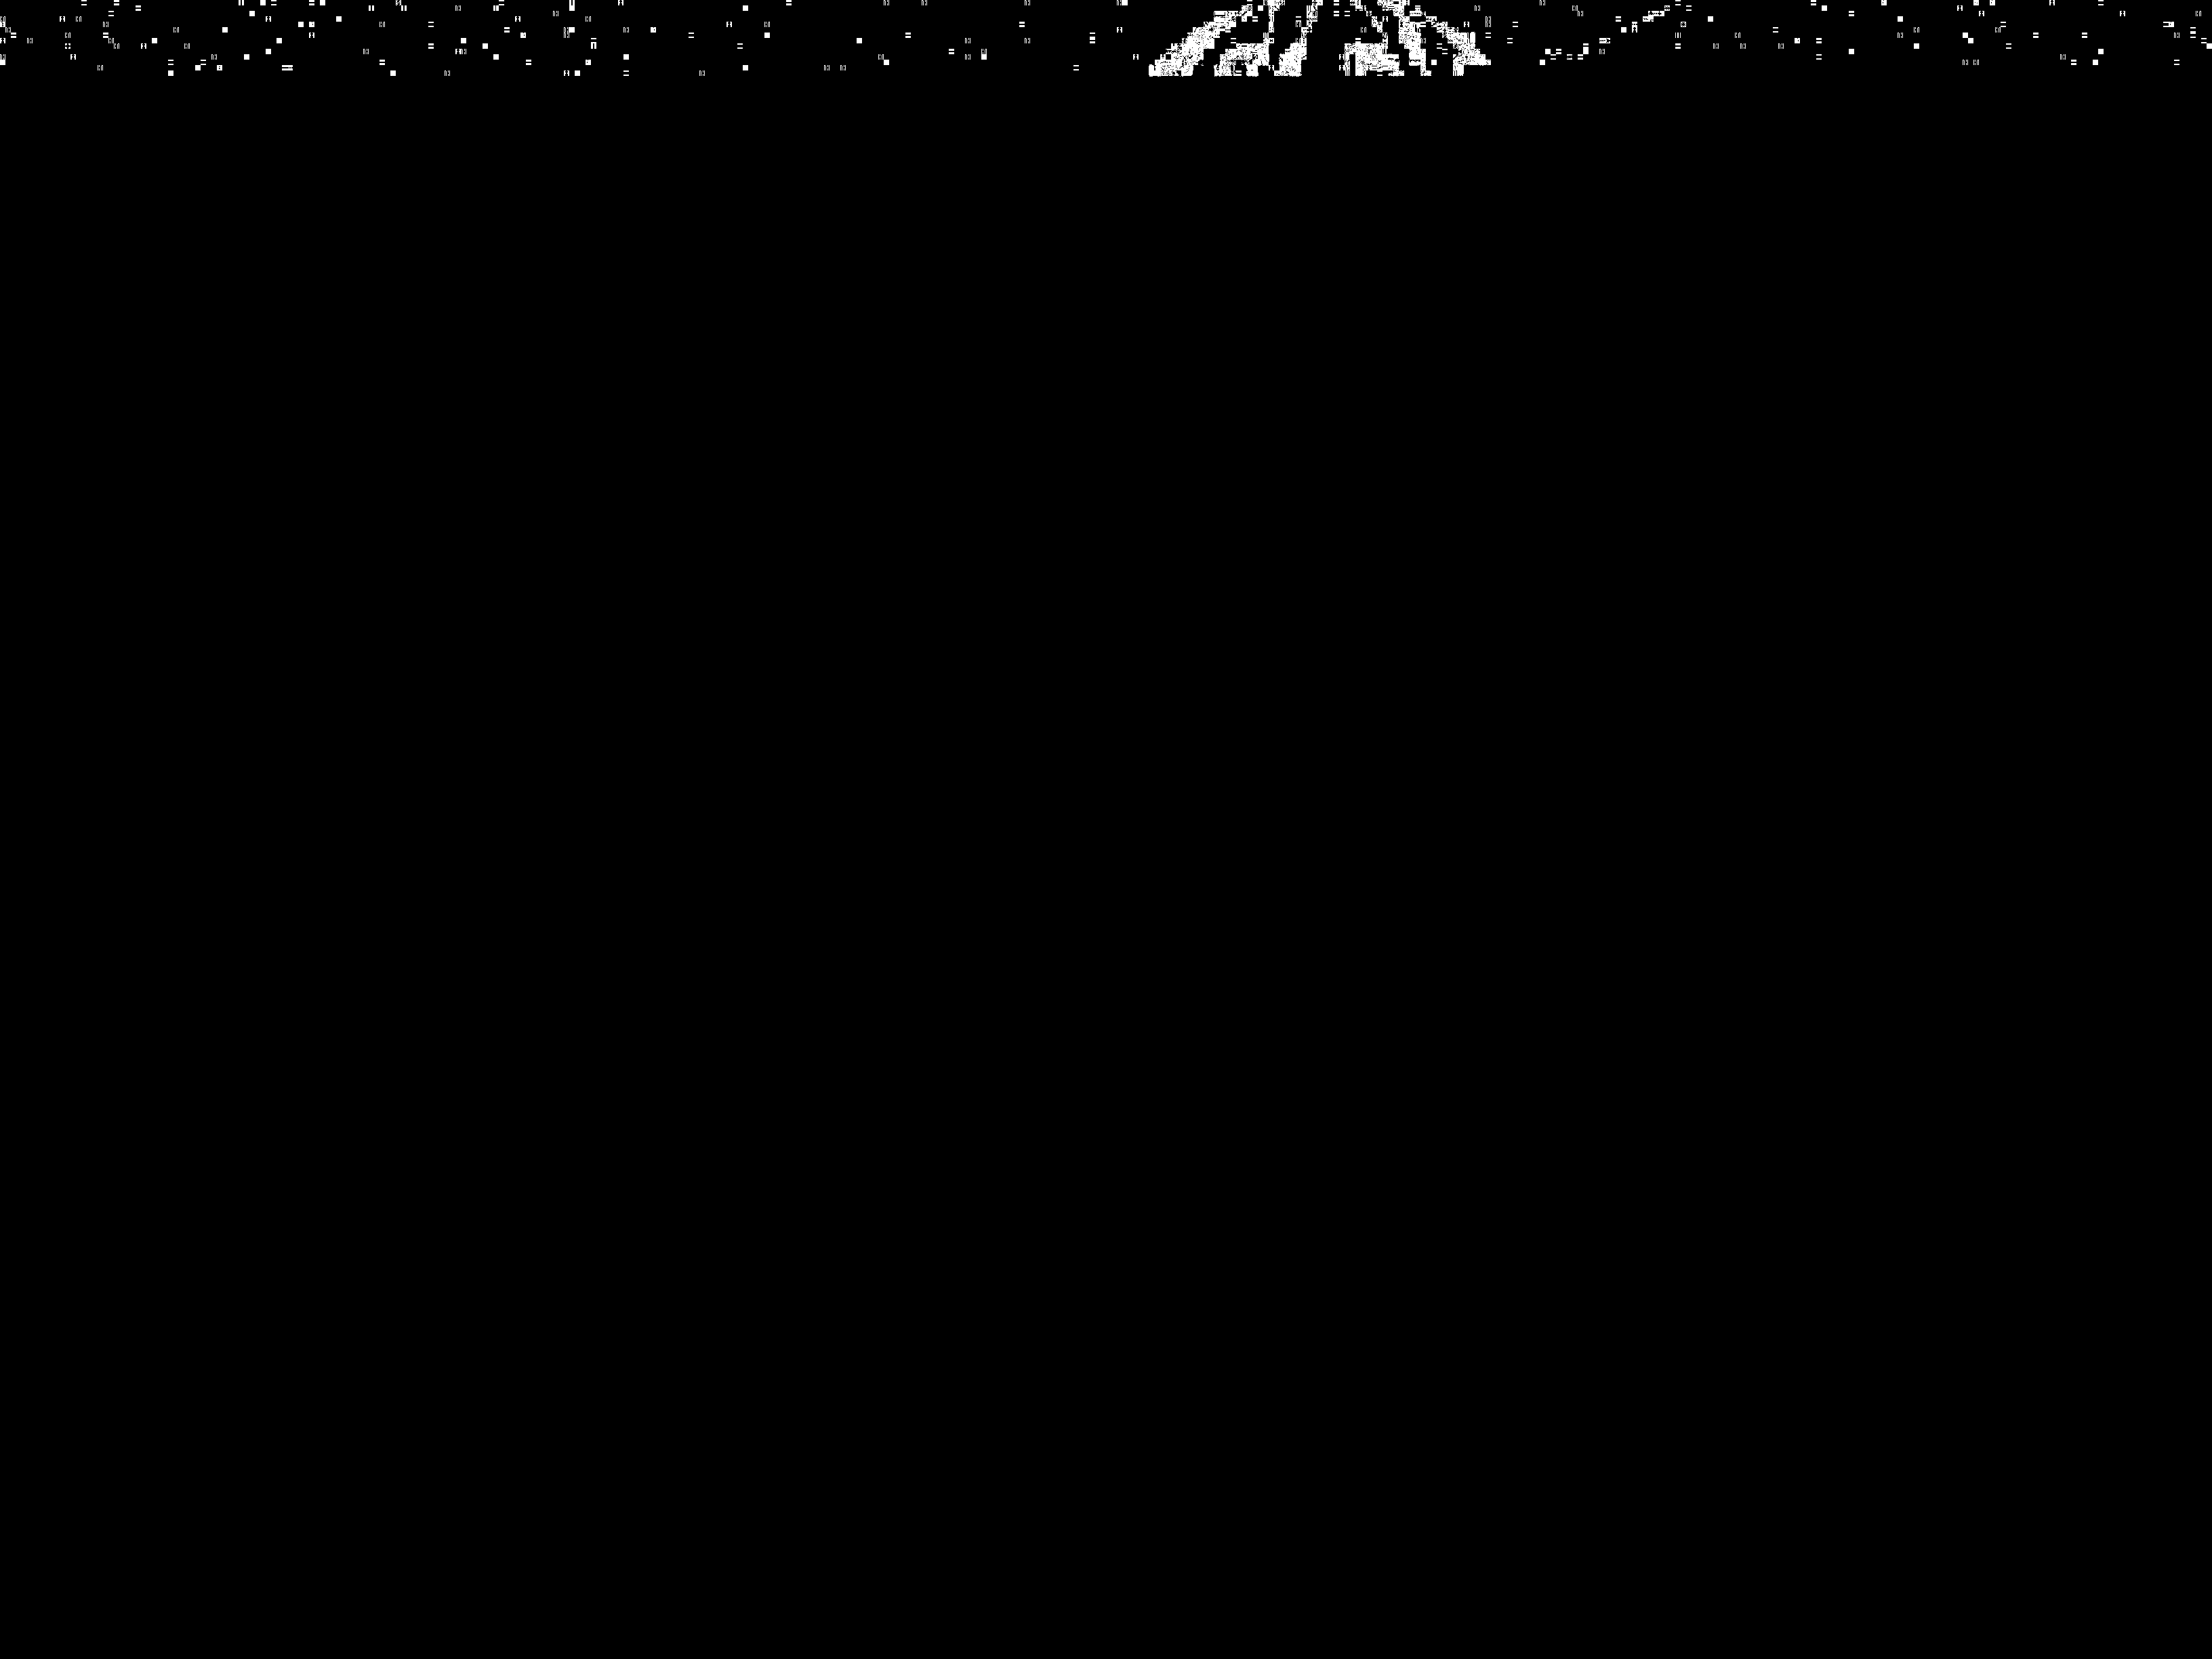
\includegraphics[width=.35\textwidth]{figures/loremIpsum1paragraphvs1chardiff.png}}
\caption{Sammenlligning af billeder}
\end{figure}
\note{Changes might just be due to compression
only changes in the top of the image is suspicious}
\end{frame}
	
\begin{frame}{LSB forstærkning}
	LSB forstærkning
	\begin{itemize}
		\item Fjern de 7 højtstående bits
		\item Alle bytes har nu værdien 0 eller 1
		\item Alle bytes ganges med 255
	\end{itemize}
\note{**Lead into next slide with ``Dette er en god måde at opdage om LSB er blevet brugt''**}
\end{frame}

\begin{frame}{LSB forstærkning}
\begin{figure}
\centering
\subfigure[Grid LSB encoded 20kb]{\label{gridLSBencode}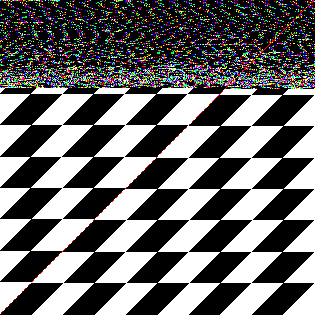
\includegraphics[width=.4\textwidth]{figures/20kbLSBencoded_LSB.png}}
\end{figure}
\note{Distortion at the top indicates something hidden in image}
\end{frame}

\begin{frame}{LSB forstærkning}
\begin{figure}
\centering
\subfigure[Original]{\label{fig:Room}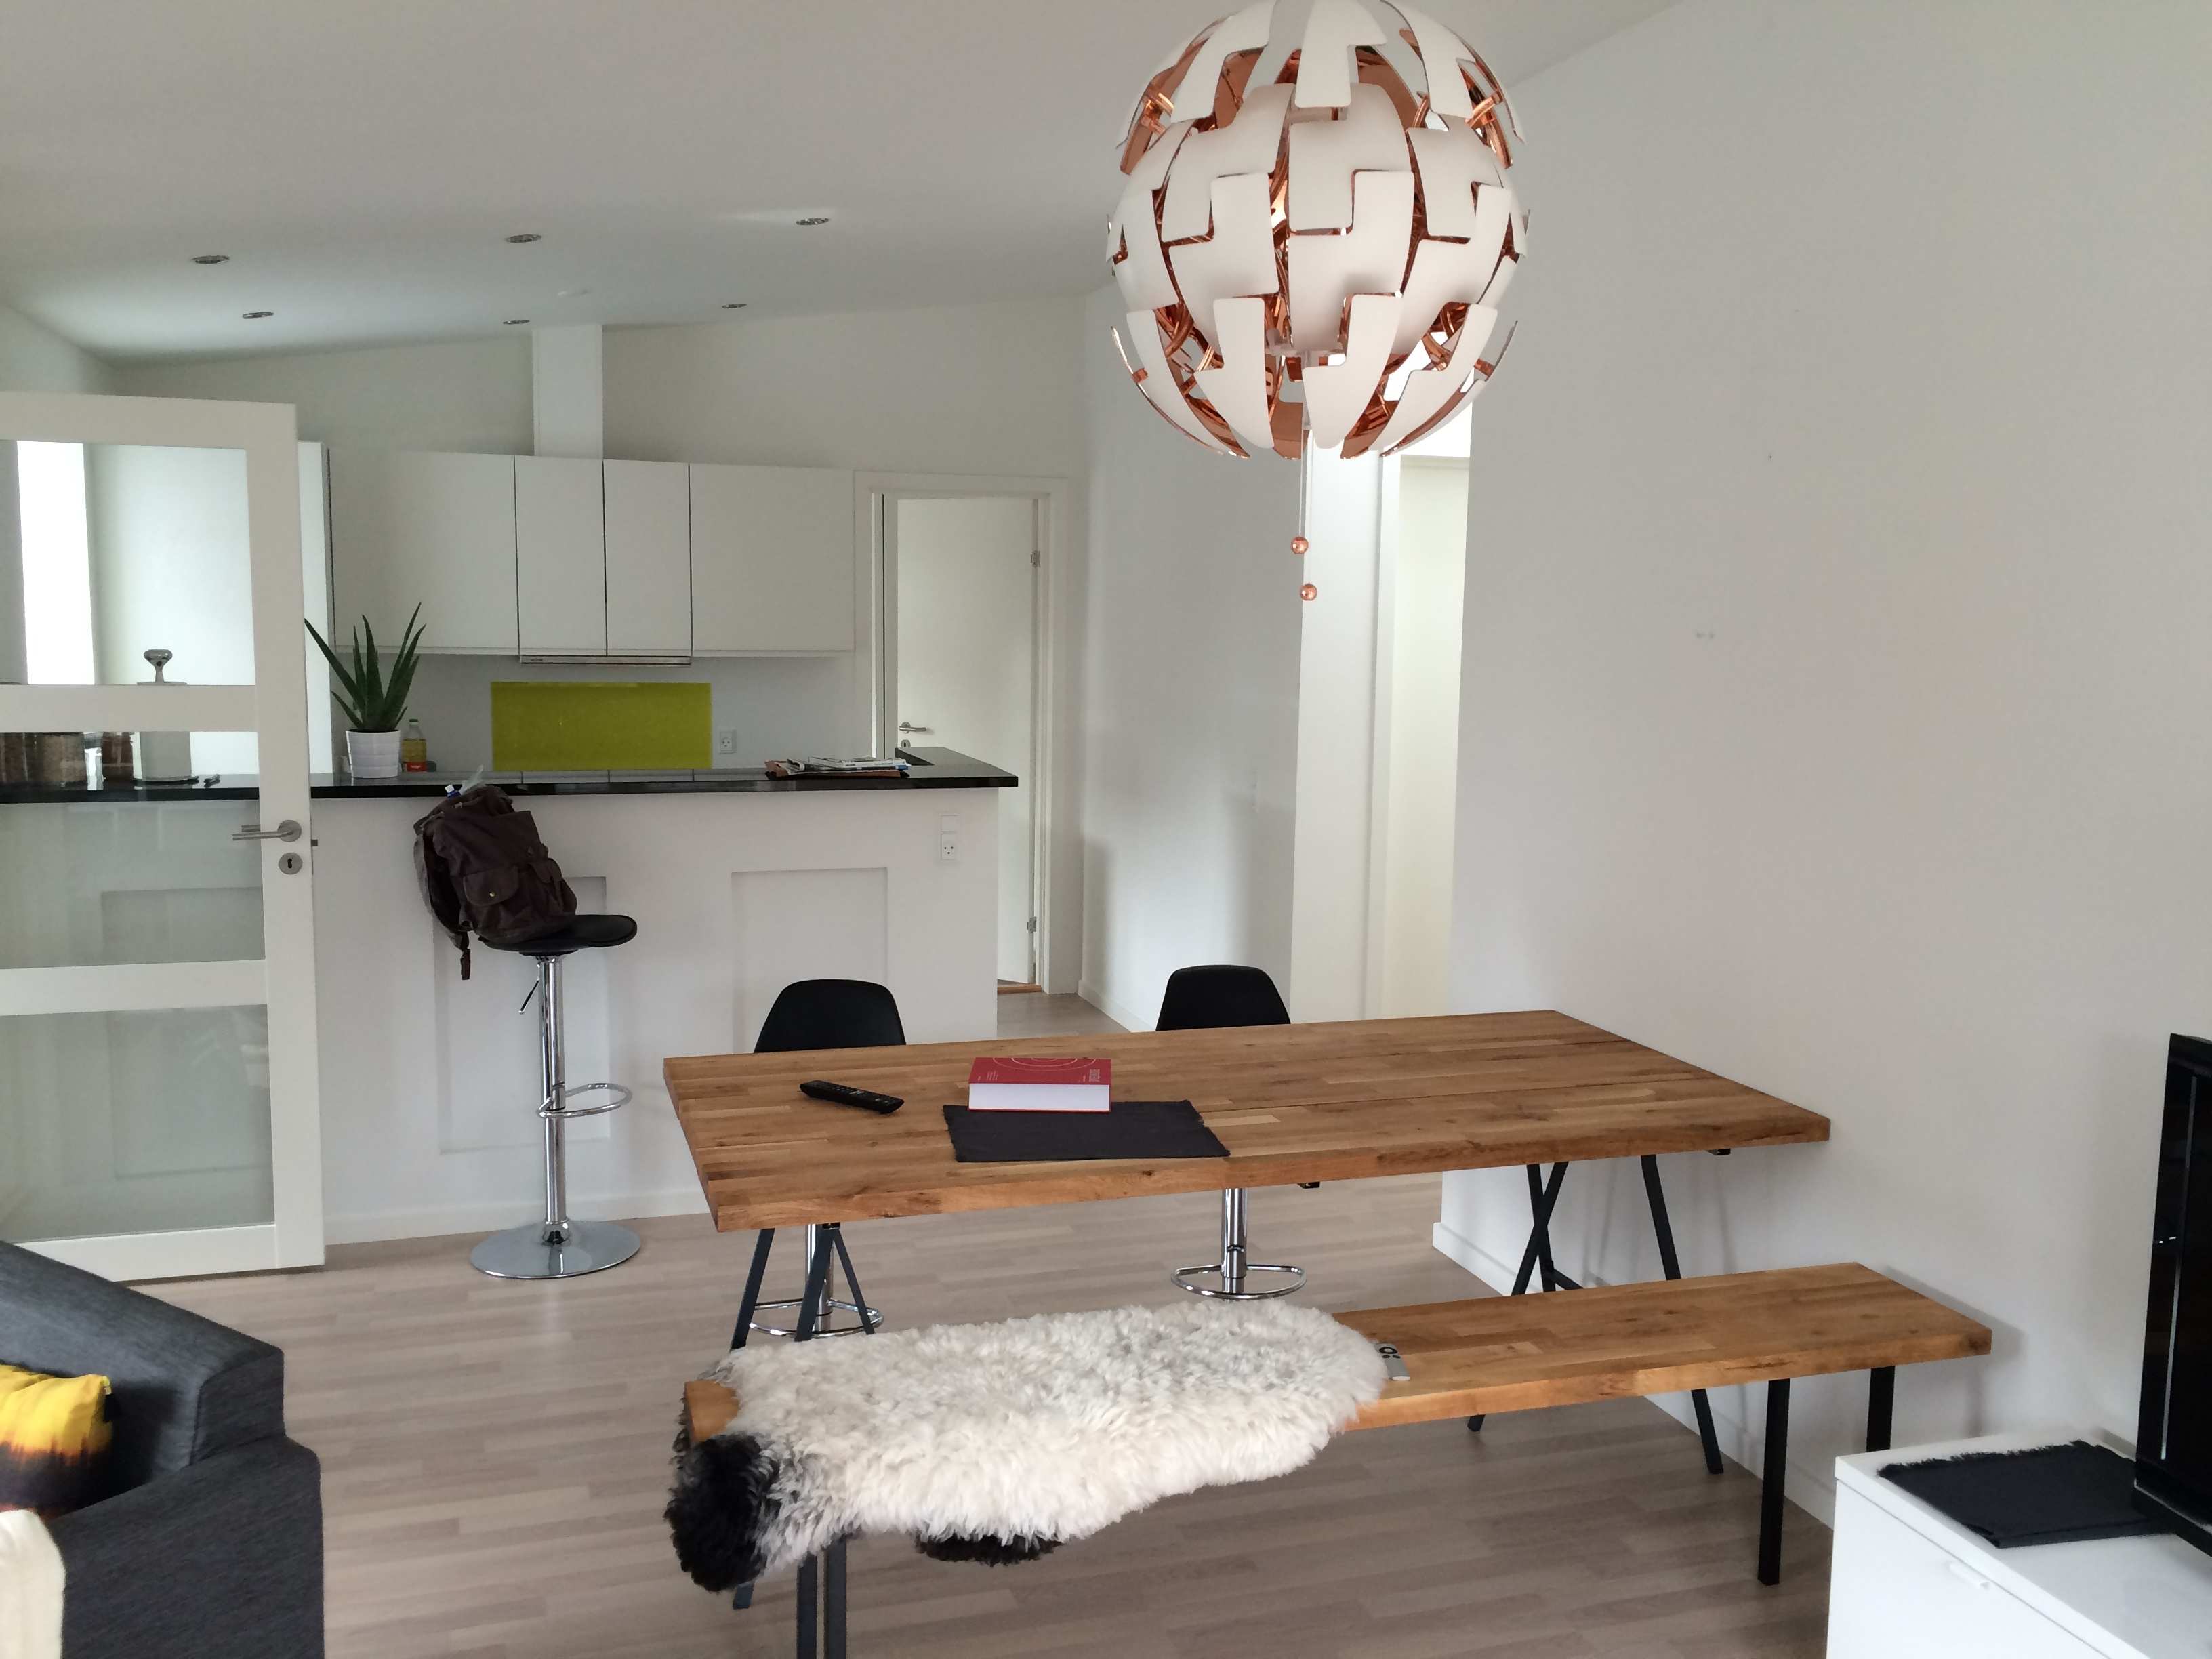
\includegraphics[width=.45\textwidth]{figures/roomOriginal.jpg}}
\subfigure[Original LSB enhanced]{\label{fig:Room}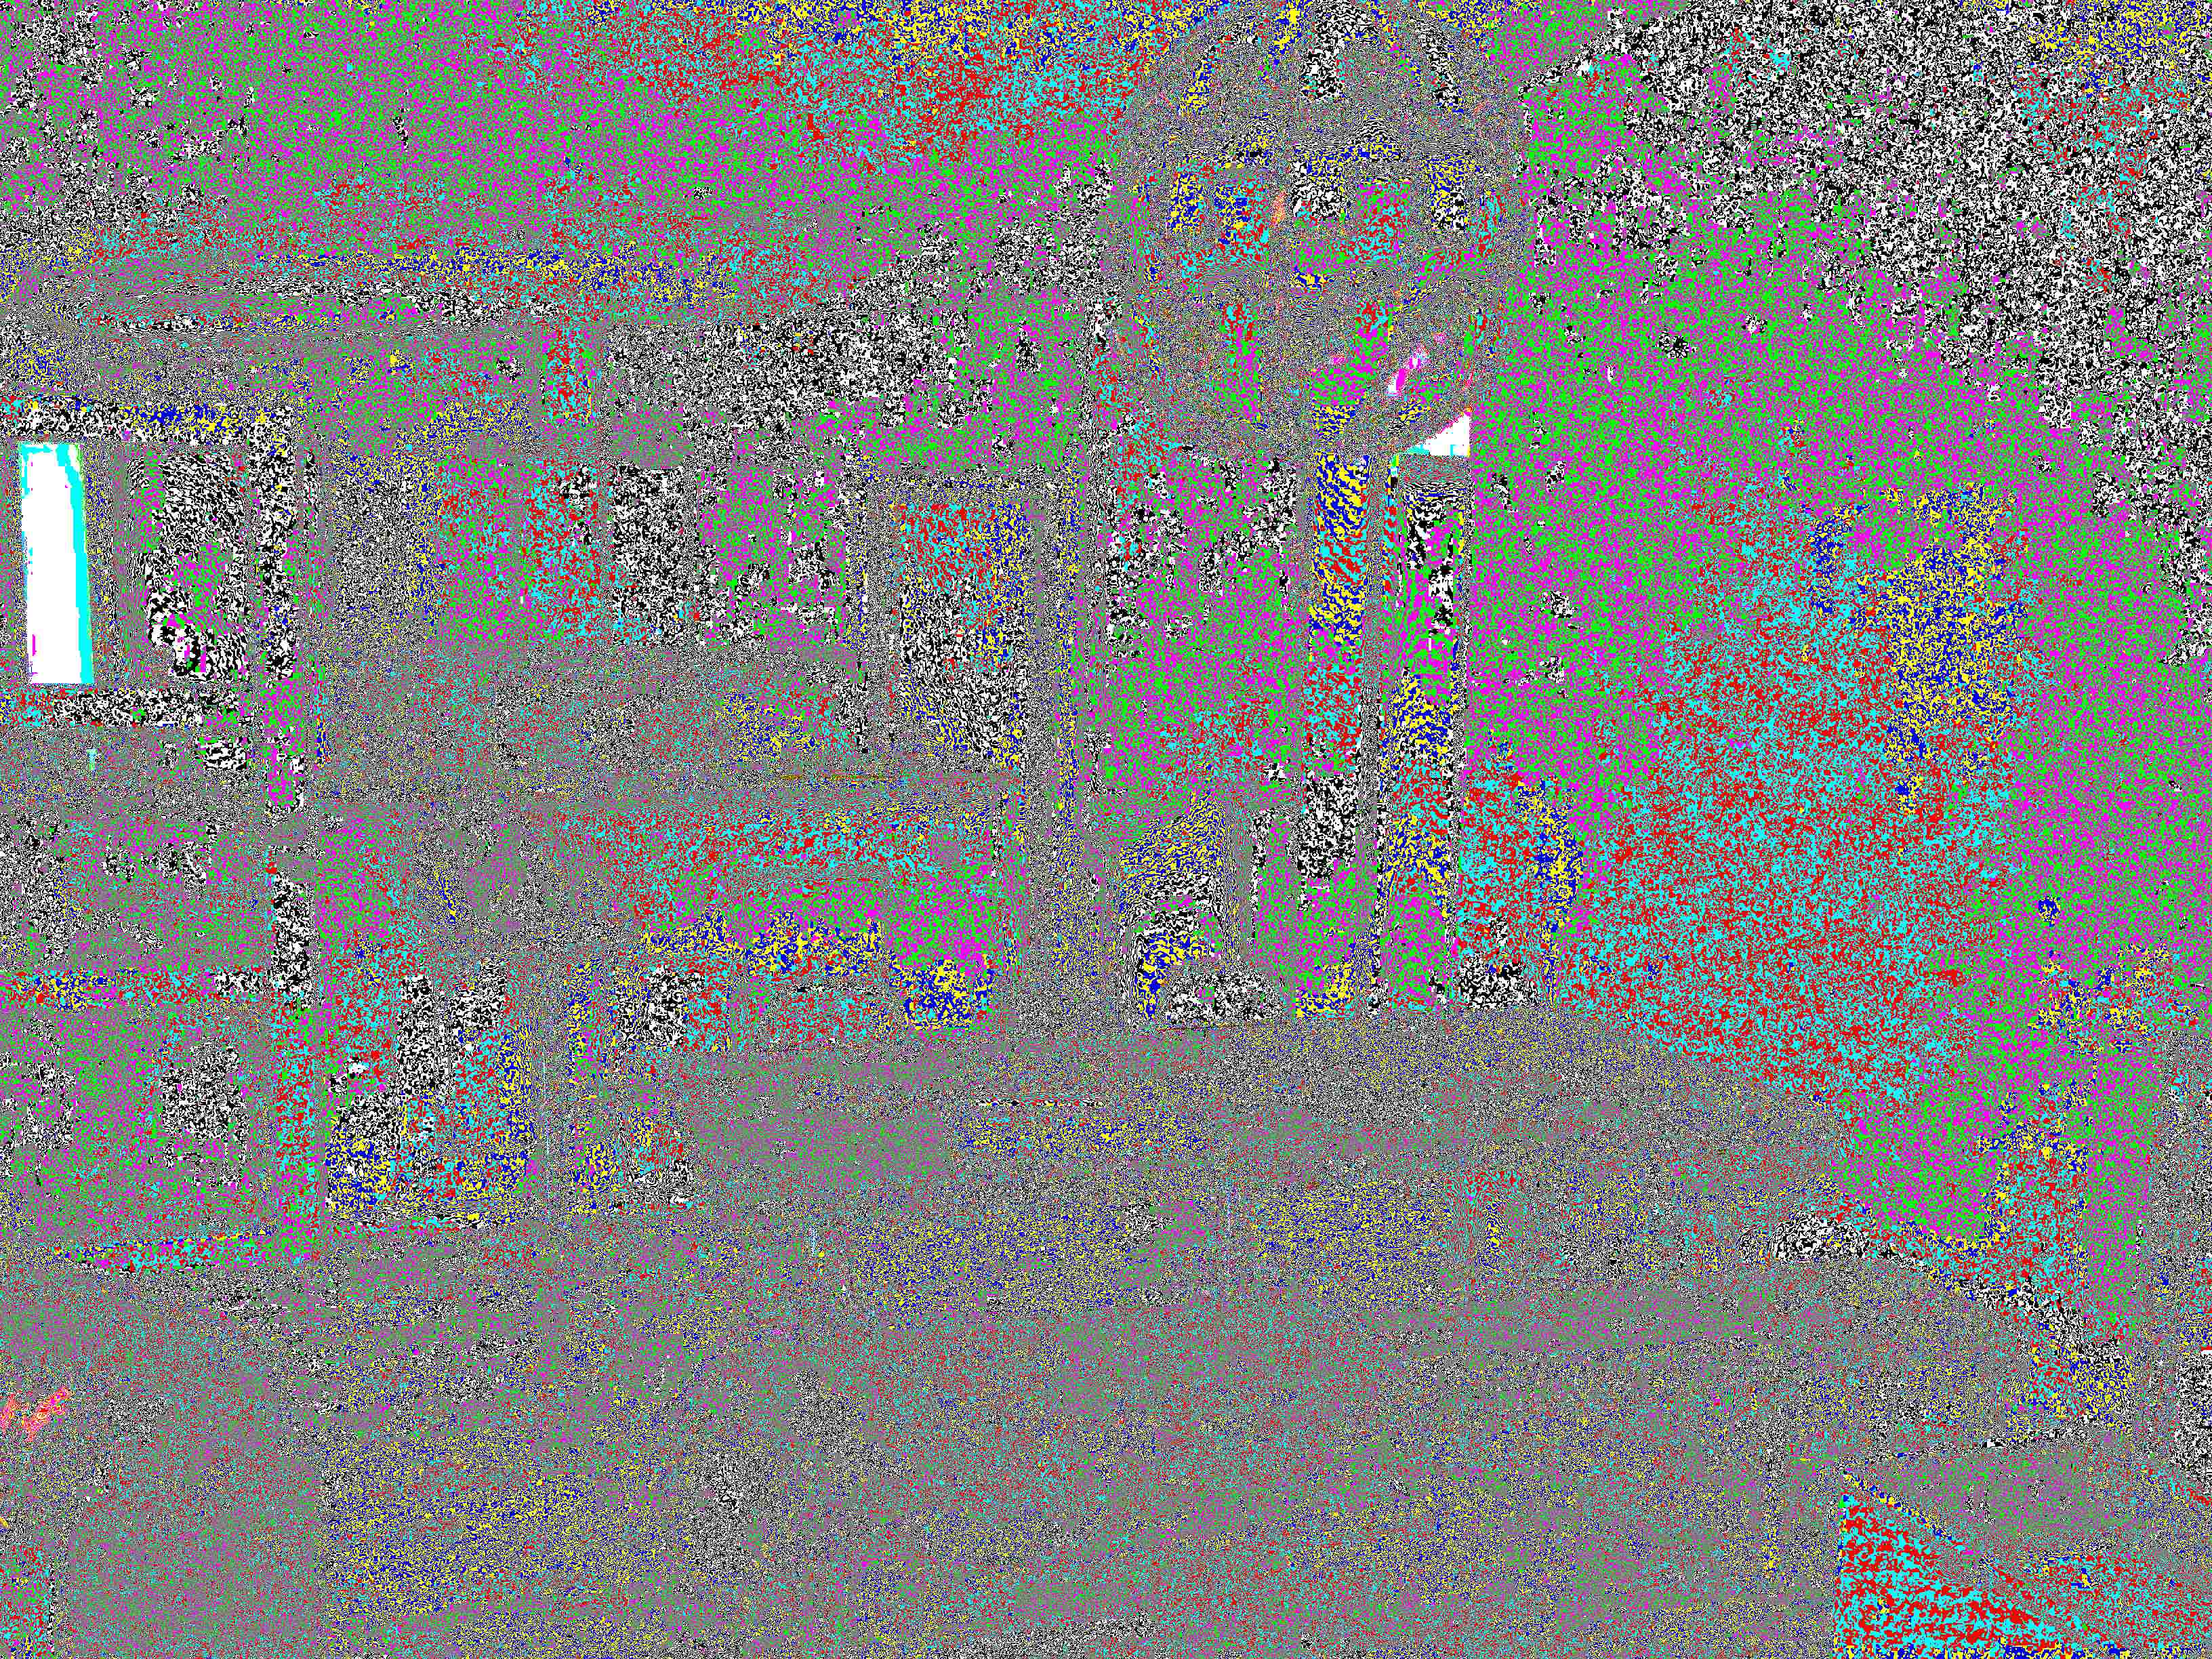
\includegraphics[width=.45\textwidth]{figures/roomOriLSB.jpg}}
\end{figure}
\note{When used on nature images, the image is giberish}
\end{frame}

\begin{frame}{LSB forstærkning}
\begin{figure}
\centering
\subfigure[Original LSB forstærket]{\label{fig:Room}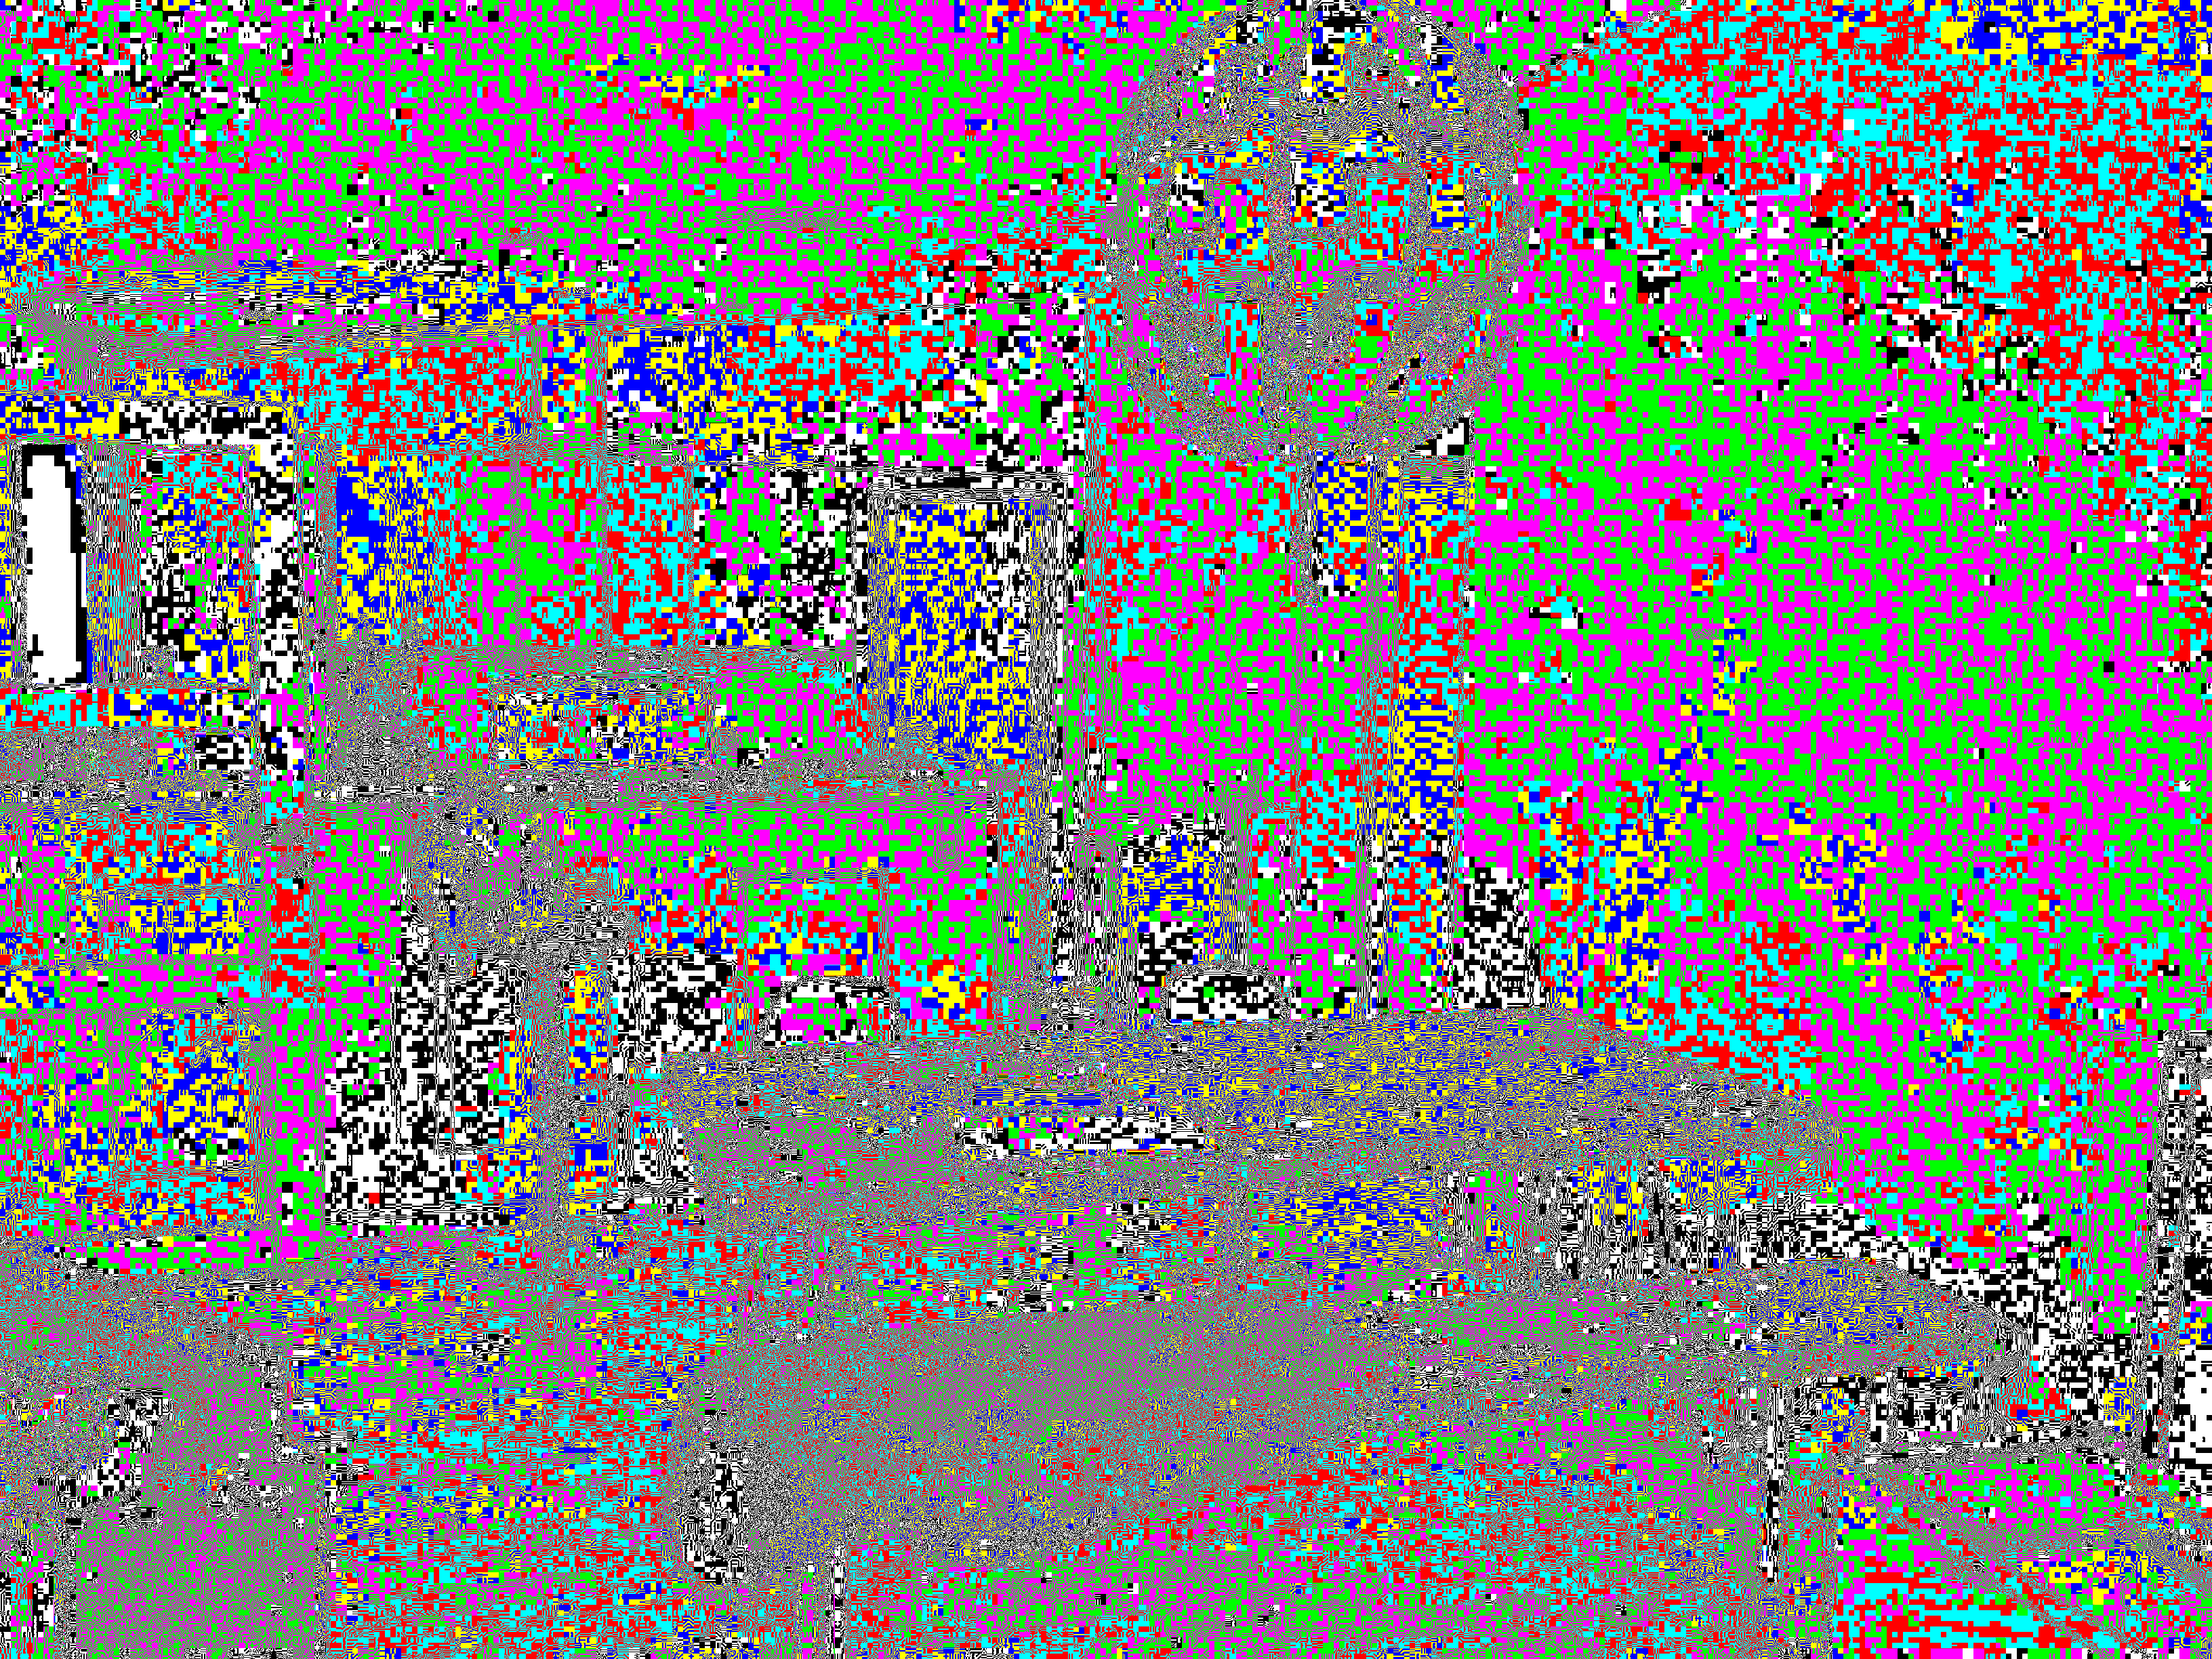
\includegraphics[width=.45\textwidth]{figures/room1charLSBEnhanced.png}}
\subfigure[2896 bytes LSB forstærket]{\label{fig:Room}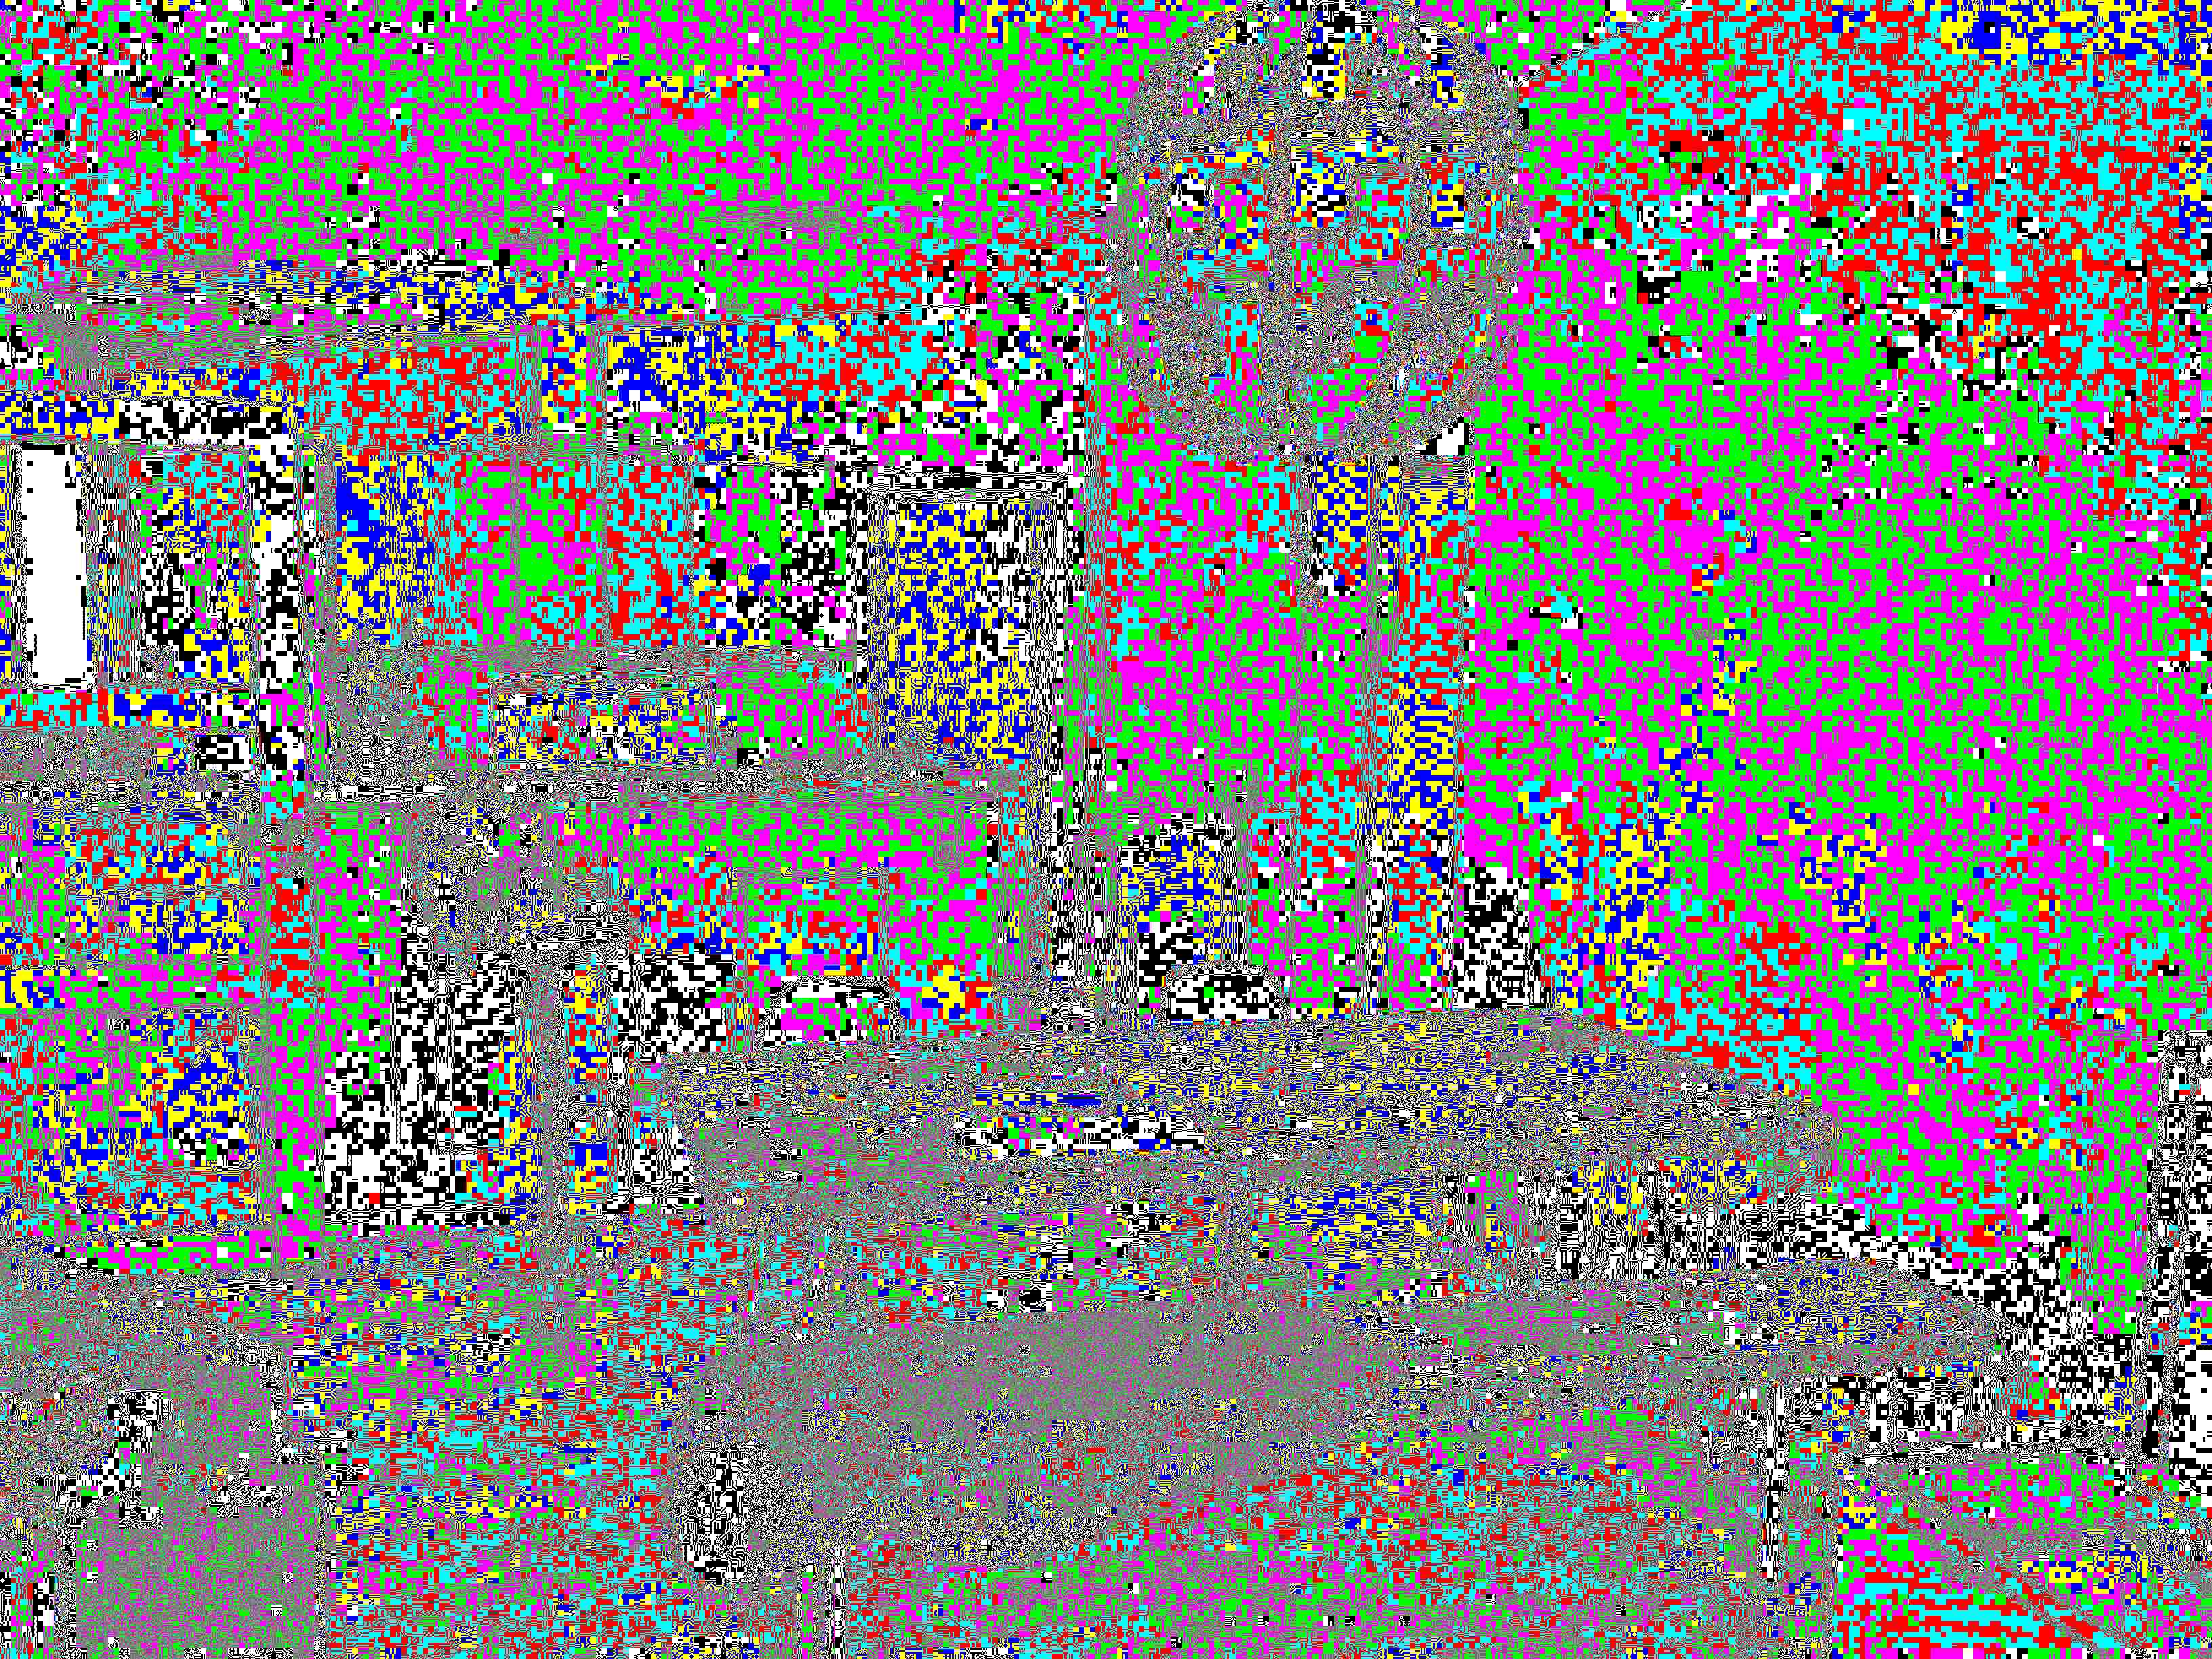
\includegraphics[width=.45\textwidth]{figures/roomIntroLSB.jpg}}
\caption{Begge billeder}
\end{figure}
\note{Looks ugly because of our JPEG encoder
While LSB enhancing works for LSB, it cannot detect our program}
\end{frame}

\begin{frame}{Signatur}
	Signatur af vores program
		\begin{itemize}
		\item Første 16 bits af scan datas ikke-nul værdier
		\item Altid indkodet med modulo 4
		\end{itemize}
\note{skip 12 bytes after scan data marker, skip zero values and skip markers. Then read the 16 bits}
\end{frame}

\begin{frame}{Brute-decoding}
	Brute-decoding
		\begin{itemize}
		\item Decode billedet uden at vide længde eller modulo
		\item Prøv alle modulo-værdier
		\end{itemize}
\note{Last ditch effort, can be somewhat automated, but is foiled by encrypting}
\end{frame}

\begin{frame}{Brute-decoding}
\begin{figure}
\centering
\subfigure[Decoded message]{\label{fig:text}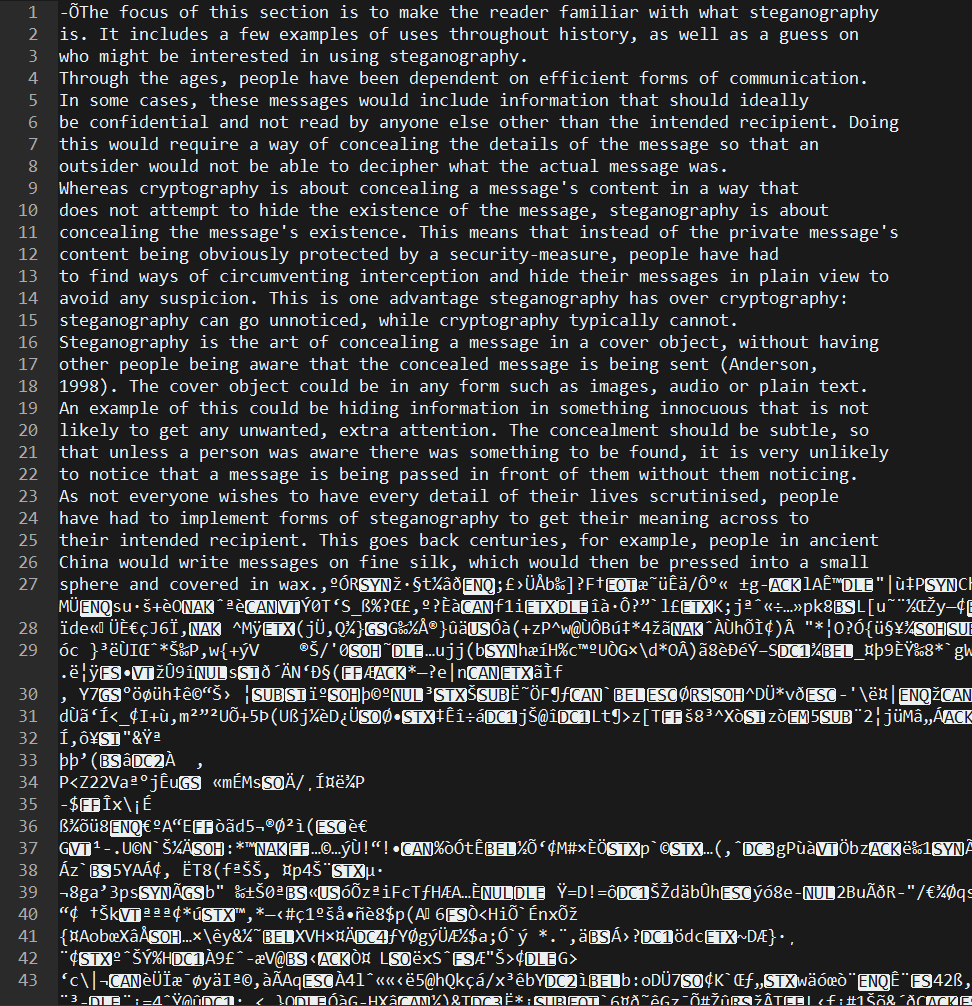
\includegraphics[width=.8\textwidth]{figures/lessGiberish.png}}
\end{figure}
\note{First 2 chars are our metaData bytes in ASCII}
\end{frame}
